\documentclass[12pt,a4paper]{article}

% ─── Packages ───────────────────────────────────────────────────────────────
\usepackage[margin=2.5cm]{geometry}
\usepackage{graphicx}
\usepackage{amsmath, amssymb, bm}
\usepackage{physics}
\usepackage{caption}
\usepackage{subcaption}
\usepackage{float}
\usepackage{booktabs}
\usepackage{array}
\usepackage{xcolor}
\usepackage{hyperref}
\usepackage{cleveref}
\usepackage{mdframed}
\usepackage{enumitem}
\usepackage{fancyhdr}
\usepackage{titlesec}
\usepackage{parskip}
\usepackage{lmodern}
\usepackage[T1]{fontenc}

% ─── Colours ────────────────────────────────────────────────────────────────
\definecolor{deepblue}{RGB}{10,60,120}
\definecolor{lightblue}{RGB}{220,235,252}
\definecolor{alertred}{RGB}{180,30,30}
\definecolor{notegreen}{RGB}{20,120,60}
\definecolor{placeholdergray}{RGB}{200,200,200}

% ─── Hyperref setup ──────────────────────────────────────────────────────────
\hypersetup{
  colorlinks=true,
  linkcolor=deepblue,
  urlcolor=deepblue,
  citecolor=notegreen
}

% ─── Header / Footer ─────────────────────────────────────────────────────────
\pagestyle{fancy}
\fancyhf{}
\fancyhead[L]{\small\textcolor{deepblue}{\textbf{Wigner Distribution Visualizer}}}
\fancyhead[R]{\small\textcolor{deepblue}{Quantum Phase-Space Tomography}}
\fancyfoot[C]{\thepage}
\renewcommand{\headrulewidth}{0.6pt}

% ─── Section colours ─────────────────────────────────────────────────────────
\titleformat{\section}{\large\bfseries\color{deepblue}}{}{0em}{\thesection\quad}
\titleformat{\subsection}{\normalsize\bfseries\color{deepblue!80}}{}{0em}{\thesubsection\quad}

% ─── Placeholder figure command ───────────────────────────────────────────────
%  Usage: \placeholder{width}{height-cm}{label text}{caption}
\newcommand{\placeholder}[4]{%
  \begin{figure}[H]
    \centering
    \fcolorbox{deepblue}{lightblue}{%
      \begin{minipage}{#1}
        \vspace{#2}
        \centering
        \textcolor{deepblue}{\large\bfseries [FIGURE PLACEHOLDER]}\\[6pt]
        \textcolor{deepblue!70}{\small #3}
        \vspace{#2}
      \end{minipage}%
    }
    \caption{#4}
  \end{figure}
}

% ─── Note / Info box ─────────────────────────────────────────────────────────
\newmdenv[
  backgroundcolor=lightblue,
  linecolor=deepblue,
  linewidth=1.5pt,
  leftmargin=0pt,
  rightmargin=0pt,
  innerleftmargin=10pt,
  innerrightmargin=10pt,
  innertopmargin=8pt,
  innerbottommargin=8pt,
]{infobox}

% ─── Where-to-find box ───────────────────────────────────────────────────────
\newmdenv[
  backgroundcolor=notegreen!10,
  linecolor=notegreen,
  linewidth=1.5pt,
  leftmargin=0pt,
  rightmargin=0pt,
  innerleftmargin=10pt,
  innerrightmargin=10pt,
  innertopmargin=8pt,
  innerbottommargin=8pt,
]{notebox}

% ─────────────────────────────────────────────────────────────────────────────
\begin{document}

% ─── TITLE PAGE ──────────────────────────────────────────────────────────────
\begin{titlepage}
  \centering
  \vspace*{2cm}
  {\Huge\bfseries\color{deepblue} Homodyne Detection and Tomography}\\[0.6em]
  {\large\color{deepblue!80} Quantum Phase-Space Distributions and Wigner Distribution Visualizer}\\[2em]
  \rule{0.6\textwidth}{1pt}\\[2em]
  \begin{tabular}{rl}
    \textbf{Tool:}    & Homodyne Detection and Tomography \\[4pt]
    \textbf{Author:}  & OM AMOL TATHED \\[4pt]
    \textbf{Roll No:}    & M25IQT009 \\[4pt]
    \textbf{Instructor:} & Prof. V Narayanan
  \end{tabular}
  \vfill
\end{titlepage}

% ─── TABLE OF CONTENTS ───────────────────────────────────────────────────────
\tableofcontents
\newpage

% ─────────────────────────────────────────────────────────────────────────────
\section{Introduction}
% ─────────────────────────────────────────────────────────────────────────────

The Wigner quasi-probability distribution function provides a complete phase-space description of a quantum-optical state. For a density operator $\hat{\rho}$, the Wigner function is defined as

\begin{equation}
  W(x,p) = \frac{1}{\pi\hbar} \int_{-\infty}^{\infty}
            \bra{x+y}\hat{\rho}\ket{x-y}\,e^{2ipy/\hbar}\,dy,
  \label{eq:wigner_def}
\end{equation}

where $x$ and $p$ are the quadrature amplitudes of the electromagnetic field. The function is real-valued and normalised,

\begin{equation}
  \iint W(x,p)\,dx\,dp = 1,
\end{equation}

but unlike classical probability distributions it can take \emph{negative} values — the hallmark of genuine quantum non-classicality. The \textit{negativity volume}

\begin{equation}
  \mathcal{N} = \iint \min\!\bigl(W(x,p),\,0\bigr)\,dx\,dp
  \label{eq:neg_volume}
\end{equation}

quantifies how non-classical a state is.

This report documents experiments performed with the \emph{Wigner Distribution Visualizer}, a Streamlit application that computes and renders $W(x,p)$ for several prototypical quantum states and simulates homodyne-detection tomography. For each experiment the relevant parameters, key equations, expected plots, and image-acquisition instructions are provided.

% ─────────────────────────────────────────────────────────────────────────────
\section{Theory}
% ─────────────────────────────────────────────────────────────────────────────

\subsection{Laguerre-Polynomial Representation}

For a state given in the Fock basis with density matrix elements $\rho_{mn}=\langle m|\hat{\rho}|n\rangle$, the Wigner function is computed via generalised Laguerre polynomials $L_n^{(\alpha)}$ \cite{leonhardt1997}:

\begin{equation}
  W(\alpha) = \frac{2}{\pi}\,e^{-2|\alpha|^2}
              \sum_{m,n} \rho_{mn}\,(-1)^m
              \sqrt{\frac{2^{n-m}\,m!}{n!}}\,
              \alpha^{n-m}\,L_m^{(n-m)}\!\bigl(4|\alpha|^2\bigr),
  \quad m \le n,
  \label{eq:laguerre}
\end{equation}

where $\alpha = x + ip$ is the complex phase-space coordinate.

\subsection{Coherent State}

A coherent state $|\alpha_0\rangle$ has the analytic Gaussian Wigner function

\begin{equation}
  W_{\rm coh}(x,p) \propto
  \exp\!\Bigl[-\bigl(x - \sqrt{2}\,\Re\alpha_0\bigr)^2
               -\bigl(p + \sqrt{2}\,\Im\alpha_0\bigr)^2\Bigr].
  \label{eq:wigner_coherent}
\end{equation}

The distribution is everywhere non-negative ($\mathcal{N}=0$).

\subsection{Vacuum Squeezed State}

For squeezing parameter $r$ and angle $\theta$:

\begin{equation}
  W_{\rm sq}(x,p) = \frac{2}{\pi}\,
    \exp\!\biggl[-2\Bigl((x\cos\theta+p\sin\theta)^2\,e^{-2r}
                         +(-x\sin\theta+p\cos\theta)^2\,e^{2r}\Bigr)\biggr].
  \label{eq:wigner_squeezed}
\end{equation}

Squeezing redistributes quantum noise between conjugate quadratures.

\subsection{Superposition (Cat) State}

A superposition of coherent states

\begin{equation}
  |\mathrm{cat}\rangle \propto \sum_k c_k |\alpha_k\rangle
  \label{eq:cat_state}
\end{equation}

exhibits interference fringes in the Wigner function whose sign alternations signal non-classicality. For the two-component even cat state $|\alpha_0\rangle+|-\alpha_0\rangle$ the fringes appear at $x=0$ with spatial frequency $4|\alpha_0|/\pi$.

\subsection{Loss Channel}

A beam-splitter with transmissivity $\eta$ maps

\begin{equation}
  W_{\rm out}(x,p) = \frac{2}{\pi(1-\eta)}
  \iint W_{\rm in}(x',p')\,
  \exp\!\left[-\frac{2\eta}{1-\eta}\left((x-\sqrt{\eta}\,x')^2+(p-\sqrt{\eta}\,p')^2\right)\right]
  dx'\,dp'.
  \label{eq:loss}
\end{equation}

Practically, the code first stretches the distribution by $1/\sqrt{\eta}$ and then convolves with a thermal kernel.

\subsection{Homodyne Tomography}

A homodyne detector measures the quadrature $x_\theta = x\cos\theta + p\sin\theta$. The marginal distribution

\begin{equation}
  \mathrm{pr}(x_\theta) = \int W(x,p)\,dp_\theta
  \label{eq:marginal}
\end{equation}

is collected for $N_\theta$ equally spaced angles $\theta\in[0°,180°)$. The sinogram $\{p(x_\theta|\theta)\}$ is inverted by filtered back-projection (FBP) to recover $W(x,p)$:

\begin{equation}
  W(x,p) = \int_0^{\pi} \mathcal{F}^{-1}\!\bigl[|\nu|\,\tilde{p}(\nu|\theta)\bigr](x\cos\theta+p\sin\theta)\,d\theta,
  \label{eq:fbp}
\end{equation}

where $\tilde{p}(\nu|\theta)$ is the Fourier transform of the marginal and $|\nu|$ is the ramp filter.

% ─────────────────────────────────────────────────────────────────────────────
\section{Experimental Results}
% ─────────────────────────────────────────────────────────────────────────────

Each subsection constitutes one \emph{experiment}: a fixed set of input parameters, the theoretical prediction, and image placeholders for the plots you must capture from the app.

% ─────────────────────────────────────
\subsection{Experiment 1 — Coherent State at Different Amplitudes}
\label{sec:exp1}
% ─────────────────────────────────────

\subsubsection*{Theoretical background}

A coherent state $|\alpha_0\rangle$ with $|\alpha_0|=A$ is displaced from the vacuum by $A$ in phase space. Because \cref{eq:wigner_coherent} is Gaussian with unit variance (in natural units), the distribution simply translates without deformation as $A$ increases.

\subsubsection*{Parameter sets}

\begin{table}[H]
  \centering
  \caption{Parameters for Coherent State experiments.}
  \label{tab:coherent_params}
  \begin{tabular}{ccccc}
    \toprule
    \textbf{Run} & $\Re(\alpha)$ & $\Im(\alpha)$ & \textbf{Grid resolution} & \textbf{Expected $\mathcal{N}$} \\
    \midrule
    1a & 0.0 & 0.0 & 150 & 0 \\
    1b & 2.0 & 0.0 & 150 & 0 \\
    1c & 2.0 & 2.0 & 150 & 0 \\
    1d & 5.0 & 0.0 & 200 & 0 \\
    \bottomrule
  \end{tabular}
\end{table}

\subsubsection*{Key formula}

Substituting into \cref{eq:wigner_coherent} for run 1b ($\alpha_0=2$):
\begin{equation}
  W(x,p) \propto \exp\!\left[-(x-2\sqrt{2})^2 - p^2\right].
  \label{eq:coh_run1b}
\end{equation}
The peak is at $(x^*,p^*)=(2\sqrt{2},0)\approx(2.83,0)$.

\subsubsection*{Figures}

\begin{figure}[H]
  \centering
  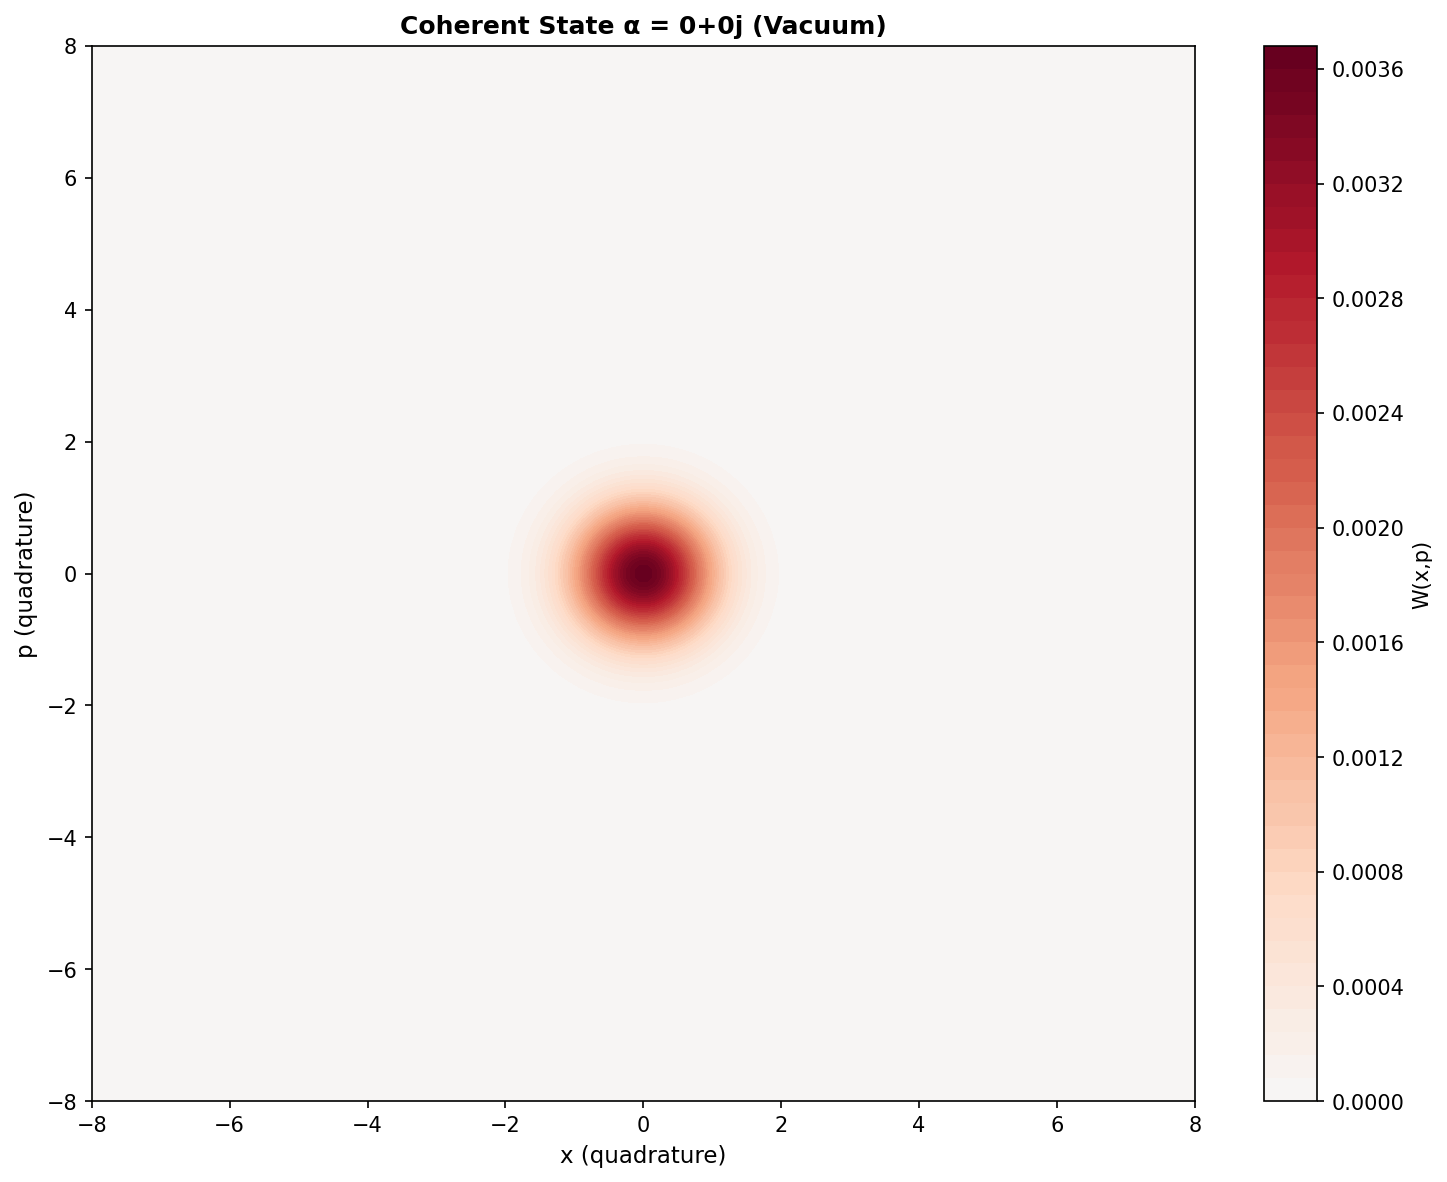
\includegraphics[width=\linewidth]{images/fig1_vacuum.png}
  \caption{Wigner distribution of the vacuum state $|0\rangle$. The distribution is a centred Gaussian, entirely non-negative ($\mathcal{N}=0$). Run 1a: $\Re(\alpha)=0$, $\Im(\alpha)=0$, res=150, no loss.}
  \label{fig:vacuum}
\end{figure}

\begin{figure}[H]
  \centering
  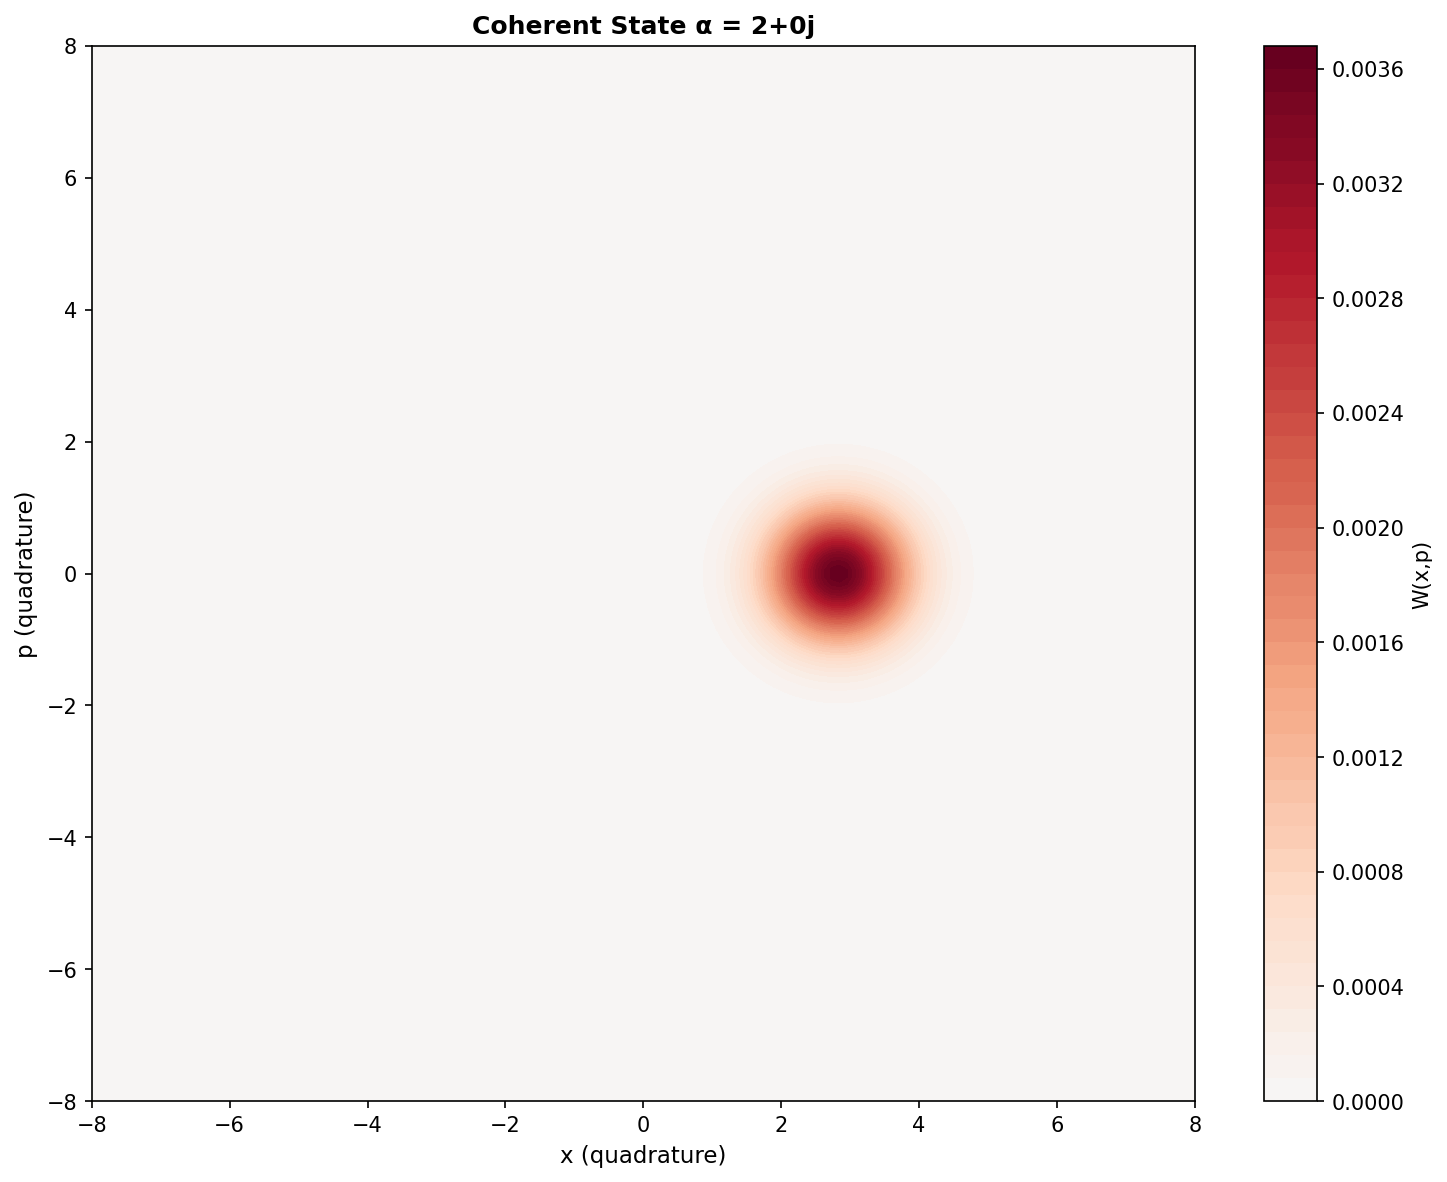
\includegraphics[width=\linewidth]{images/fig2_coh_alpha2.png}
  \caption{Wigner distribution for Run 1b ($\alpha_0=2$). The Gaussian is displaced to $(2\sqrt{2},0)\approx(2.83,0)$ in phase space. Parameters: $\Re(\alpha)=2$, $\Im(\alpha)=0$, res=150, no loss.}
  \label{fig:coh_alpha2}
\end{figure}

\begin{figure}[H]
  \centering
  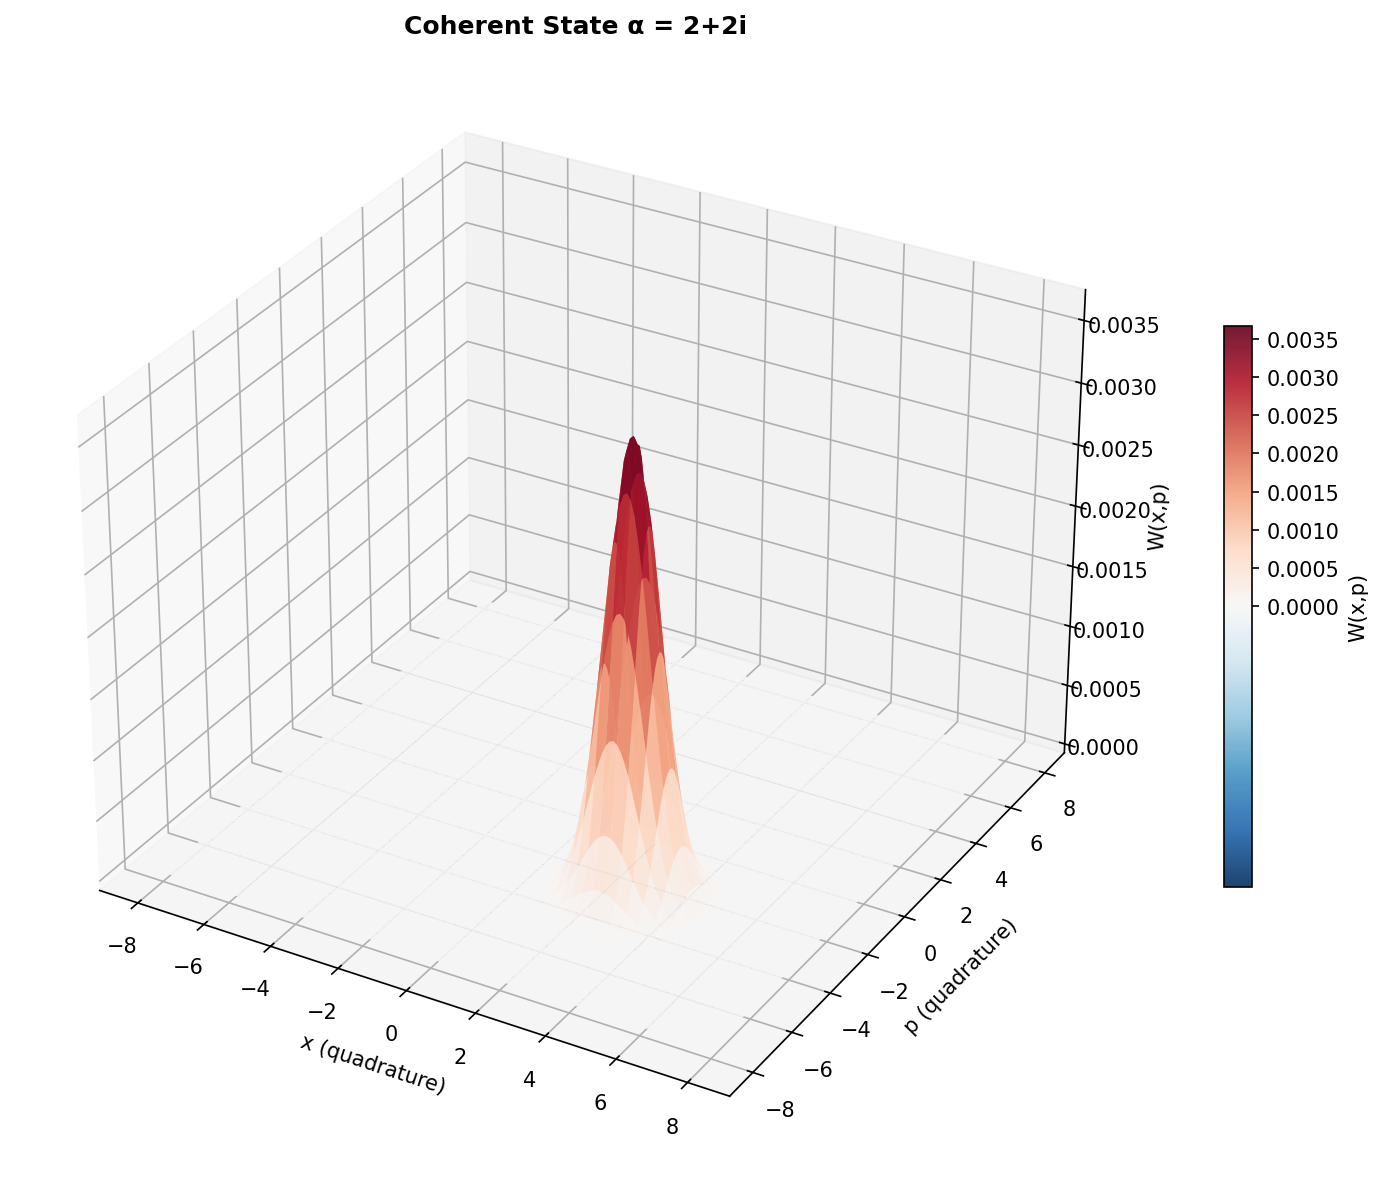
\includegraphics[width=\linewidth]{images/fig3_coh_alpha2+2i_3D.png}
  \caption{Three-dimensional Wigner surface for the coherent state displaced in both quadratures (Run 1c). The Gaussian peak sits at $(2\sqrt{2},-2\sqrt{2})\approx(2.83,-2.83)$. Parameters: $\Re(\alpha)=2$, $\Im(\alpha)=2$, res=150, no loss.}
  \label{fig:coh_alpha2+2i_3D}
\end{figure}

% ─────────────────────────────────────
\subsection{Experiment 2 — Vacuum Squeezed State}
\label{sec:exp2}
% ─────────────────────────────────────

\subsubsection*{Theoretical background}

The Heisenberg uncertainty relation $\Delta x\,\Delta p \ge 1/2$ is saturated for coherent states with $\Delta x=\Delta p=1/\sqrt{2}$. A squeezed state reduces $\Delta x_\theta$ below the vacuum level at the cost of increased $\Delta p_\theta$:

\begin{equation}
  \Delta x_\theta = \frac{1}{\sqrt{2}}\,e^{-r}, \qquad
  \Delta p_\theta = \frac{1}{\sqrt{2}}\,e^{+r}.
\end{equation}

\subsubsection*{Parameter sets}

\begin{table}[H]
  \centering
  \caption{Parameters for Vacuum Squeezed State experiments.}
  \label{tab:squeezed_params}
  \begin{tabular}{ccccc}
    \toprule
    \textbf{Run} & $r$ & $\theta$ (°) & \textbf{Resolution} & \textbf{Expected $\mathcal{N}$} \\
    \midrule
    2a & 0.0  & 0   & 150 & 0 \\
    2b & 1.0  & 0   & 150 & 0 \\
    2c & 2.0  & 0   & 150 & 0 \\
    2d & 1.0  & 45  & 150 & 0 \\
    2e & 1.5  & 90  & 150 & 0 \\
    \bottomrule
  \end{tabular}
\end{table}

\subsubsection*{Key formula}

For run 2b ($r=1$, $\theta=0°$), \cref{eq:wigner_squeezed} becomes
\begin{equation}
  W_{\rm 2b}(x,p) = \frac{2}{\pi}\exp\!\bigl(-2x^2 e^{-2}-2p^2 e^{2}\bigr)
                   = \frac{2}{\pi}\exp\!\bigl(-0.271\,x^2 - 14.78\,p^2\bigr).
\end{equation}
The aspect ratio of the ellipse is $e^{2r}=e^2\approx7.39$.

\subsubsection*{Figures}

\begin{figure}[H]
  \centering
  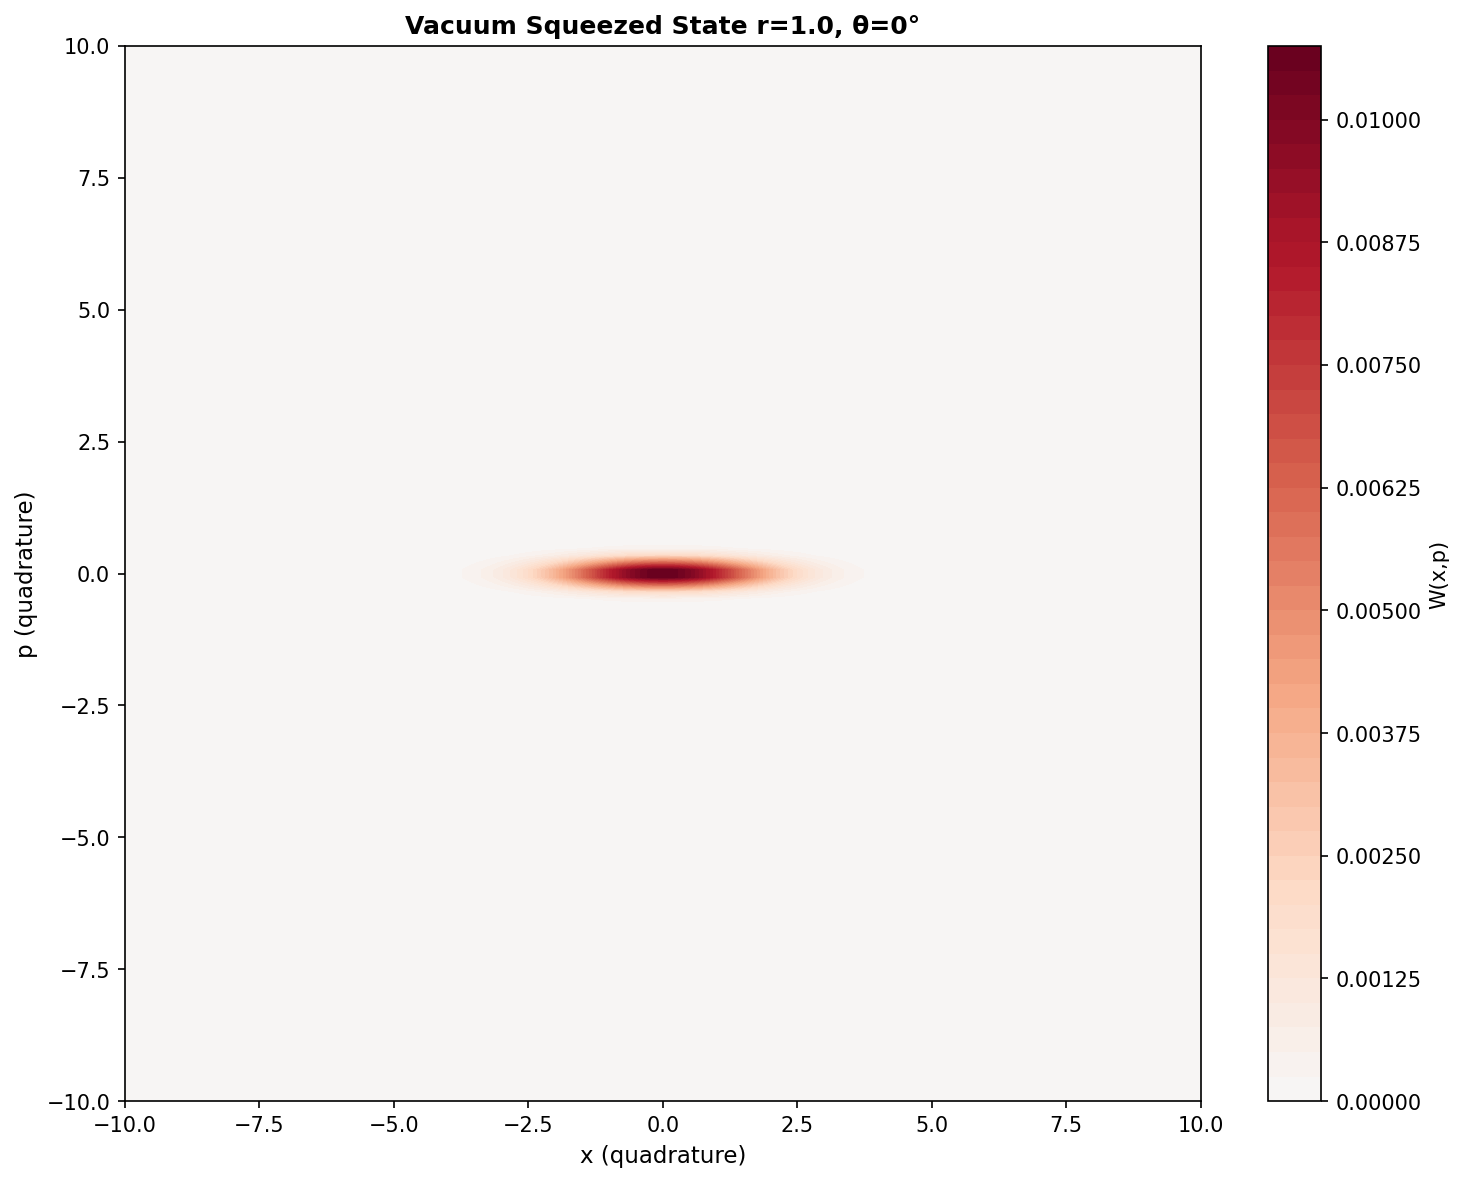
\includegraphics[width=\linewidth]{images/fig4_squeezed_r1_th0.png}
  \caption{Wigner distribution of a vacuum-squeezed state with $r=1$, $\theta=0°$ (Run 2b). The ellipse is elongated along the $x$-axis and compressed along $p$. The aspect ratio is $e^{2r}=e^2\approx7.39$.}
  \label{fig:squeezed_r1_th0}
\end{figure}

\begin{figure}[H]
  \centering
  \begin{subfigure}[b]{0.48\linewidth}
    \centering
    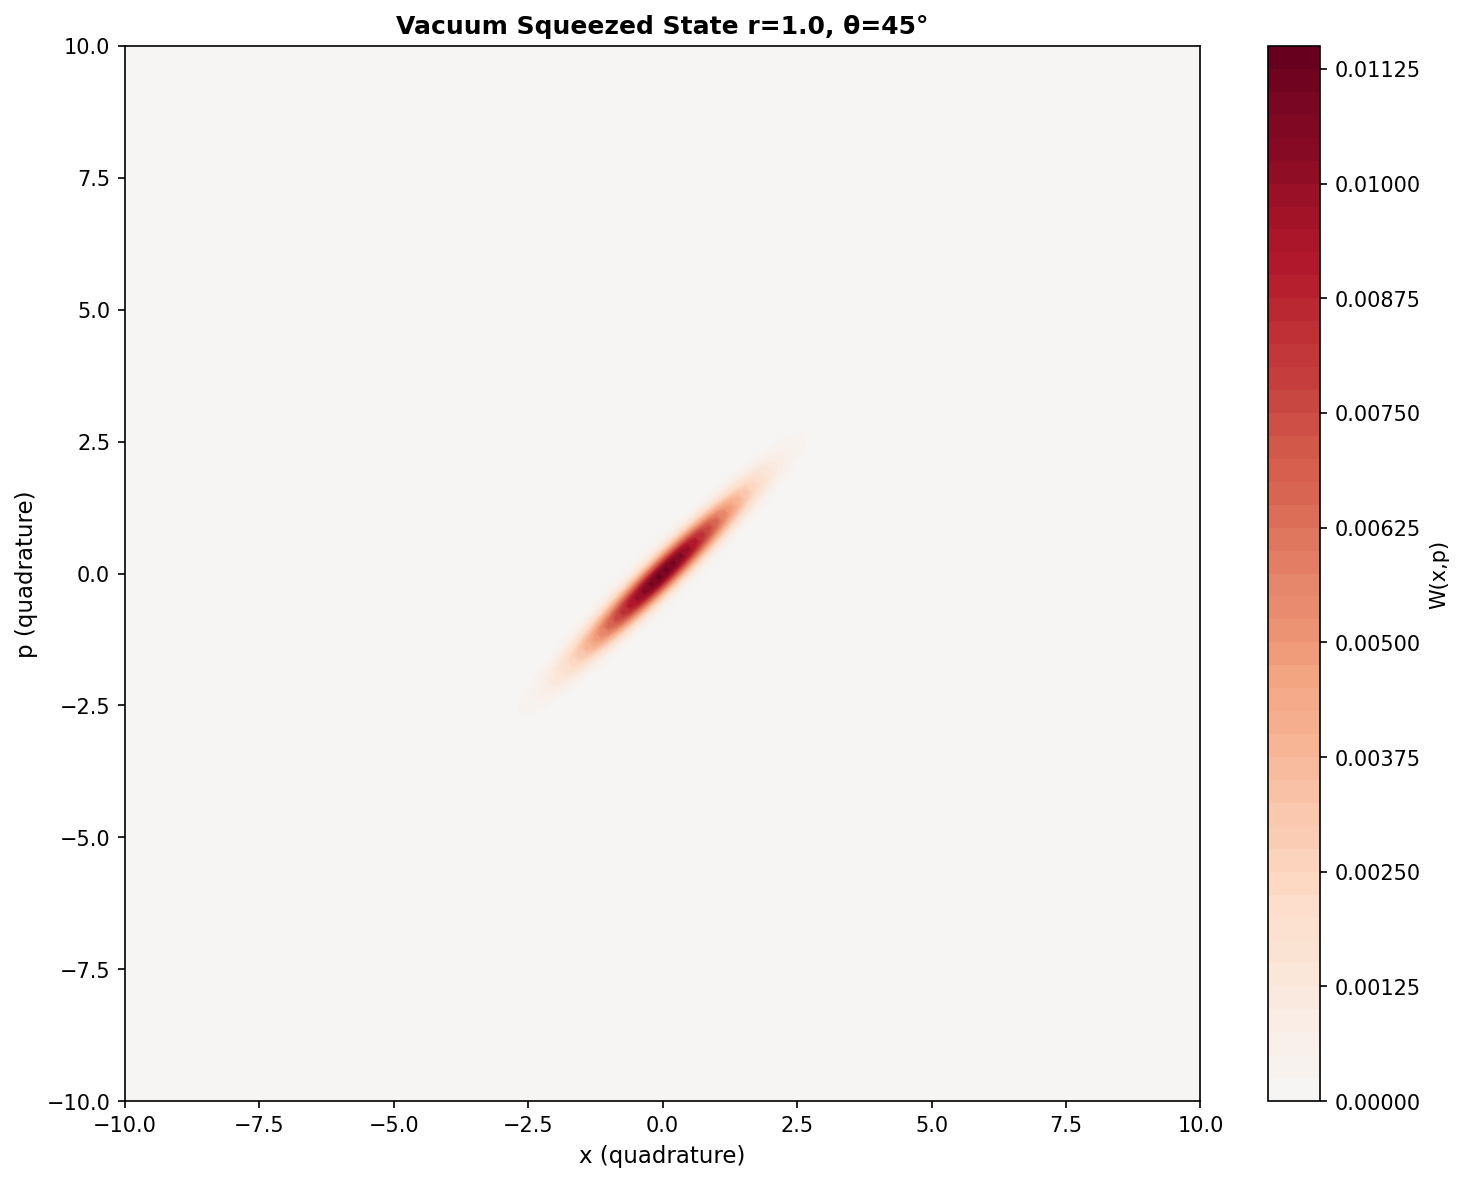
\includegraphics[width=\linewidth]{images/fig5a_squeezed_r1_th45.png}
    \caption{Rotated squeezed state, $\theta=45°$.}
  \end{subfigure}
  \hfill
  \begin{subfigure}[b]{0.48\linewidth}
    \centering
    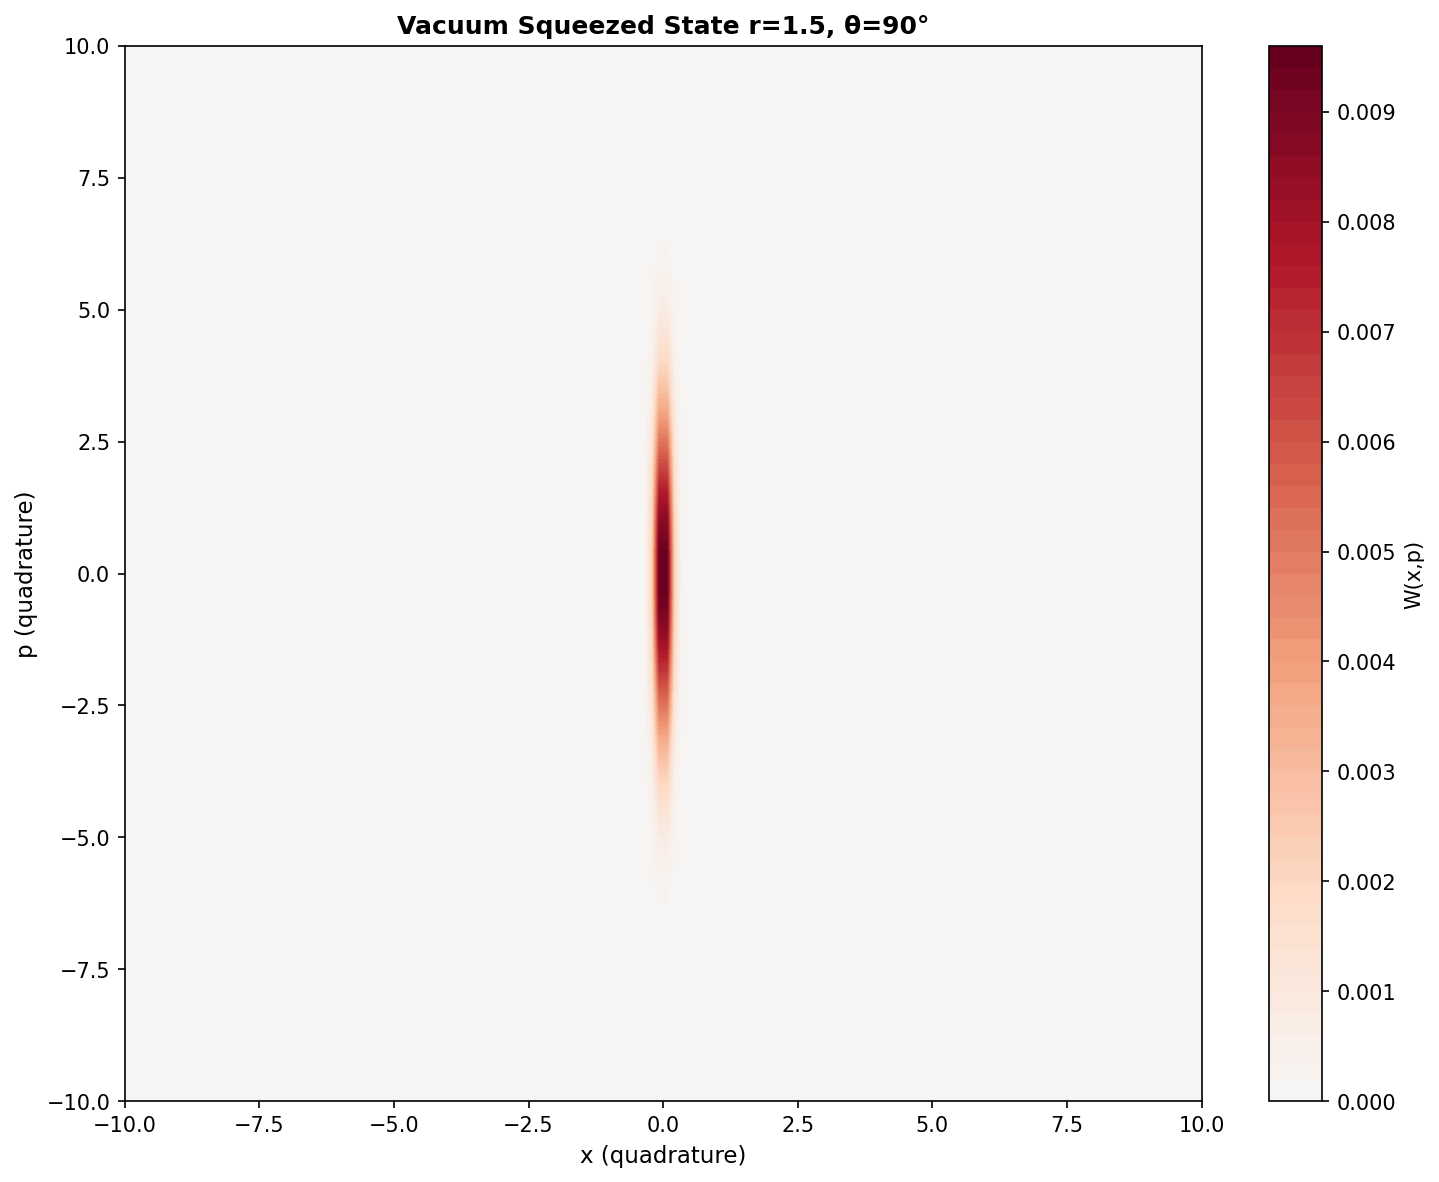
\includegraphics[width=\linewidth]{images/fig5b_squeezed_r1p5_th90.png}
    \caption{$p$-squeezed state, $\theta=90°$, $r=1.5$.}
  \end{subfigure}
  \caption{Comparison of squeezed states at different squeezing angles. Left (Run 2d): ellipse rotated $45°$ in phase space. Right (Run 2e): squeezing along the $p$-quadrature, with compression factor $e^{-1.5}\approx0.22$.}
  \label{fig:squeezed_comparison}
\end{figure}

% ─────────────────────────────────────
\subsection{Experiment 3 — Fock States}
\label{sec:exp3}
% ─────────────────────────────────────

\subsubsection*{Theoretical background}

A Fock (number) state $|n\rangle$ has the Wigner function
\begin{equation}
  W_n(x,p) = \frac{(-1)^n}{\pi}\,e^{-2|\alpha|^2}\,L_n\!\bigl(4|\alpha|^2\bigr),
  \quad |\alpha|^2=x^2+p^2,
  \label{eq:fock_wigner}
\end{equation}
where $L_n$ is the $n$-th Laguerre polynomial. The distribution has circular symmetry and exhibits $n$ nodal rings where $W<0$. The negativity volume grows monotonically with $n$.

\subsubsection*{Parameter sets}

\begin{table}[H]
  \centering
  \caption{Parameters for Fock state experiments. Fock truncation $N=20$ for all runs.}
  \label{tab:fock_params}
  \begin{tabular}{cllc}
    \toprule
    \textbf{Run} & \textbf{State vector (comma-separated)} & \textbf{State} & \textbf{Expected $\mathcal{N}$}\\
    \midrule
    3a & \texttt{1,0,0,0,0,0,0,0,0,0} & $|0\rangle$ & 0 \\
    3b & \texttt{0,1,0,0,0,0,0,0,0,0} & $|1\rangle$ & $>0$ \\
    3c & \texttt{0,0,1,0,0,0,0,0,0,0} & $|2\rangle$ & $>0$ \\
    3d & \texttt{0,0,0,0,1,0,0,0,0,0} & $|4\rangle$ & $>0$ \\
    3e & \texttt{0,0,0,0,0,0,0,1,0,0} & $|7\rangle$ & $>0$ \\
    \bottomrule
  \end{tabular}
\end{table}

\subsubsection*{Key formula}

The negativity volume for $|n\rangle$ can be estimated analytically:
\begin{equation}
  \mathcal{N}_{|n\rangle} \approx
  \begin{cases}
    0 & n=0,\\
    \dfrac{(-1)^n - 1}{2\pi} & n\ge1 \text{ (rough bound)}.
  \end{cases}
\end{equation}
A more precise result requires numerical integration of \cref{eq:neg_volume}.

\subsubsection*{Figures}

\begin{figure}[H]
  \centering
  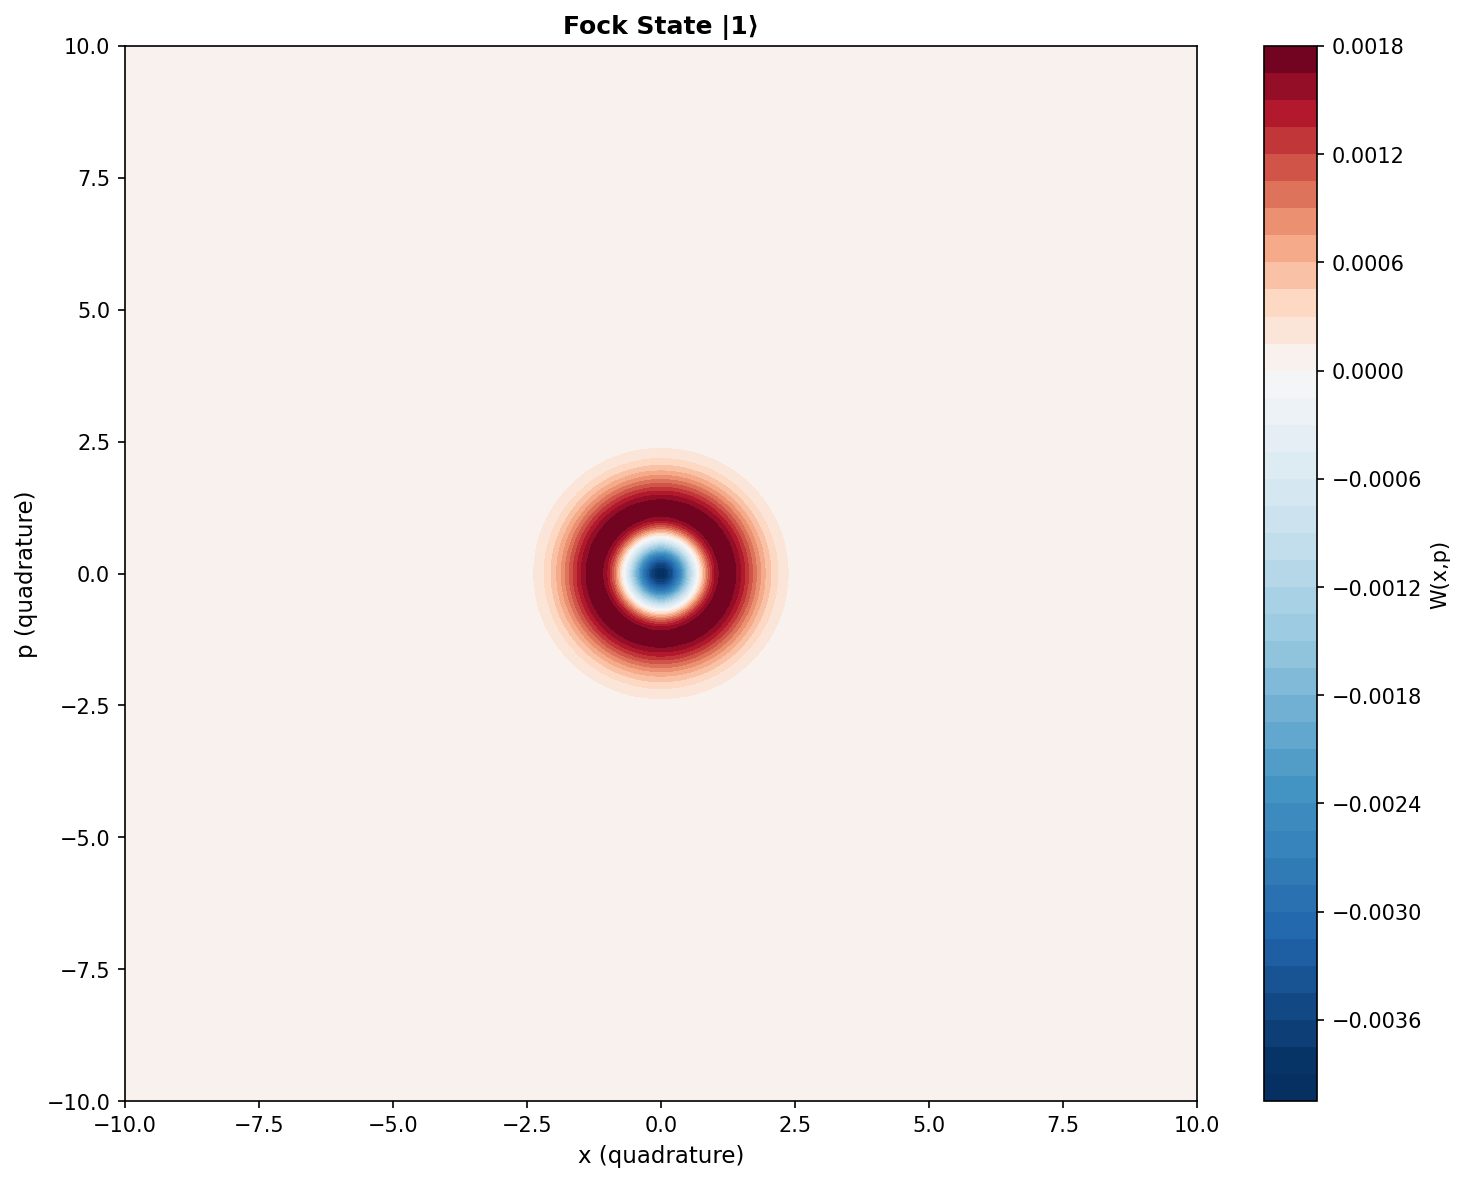
\includegraphics[width=\linewidth]{images/fig6_fock1.png}
  \caption{Wigner distribution of the single-photon Fock state $|1\rangle$ (Run 3b). The rotationally-symmetric distribution has a negative central region, confirming non-classicality. Fock truncation $N=20$, state vector \texttt{0,1,0,...,0}.}
  \label{fig:fock1}
\end{figure}

\begin{figure}[H]
  \centering
  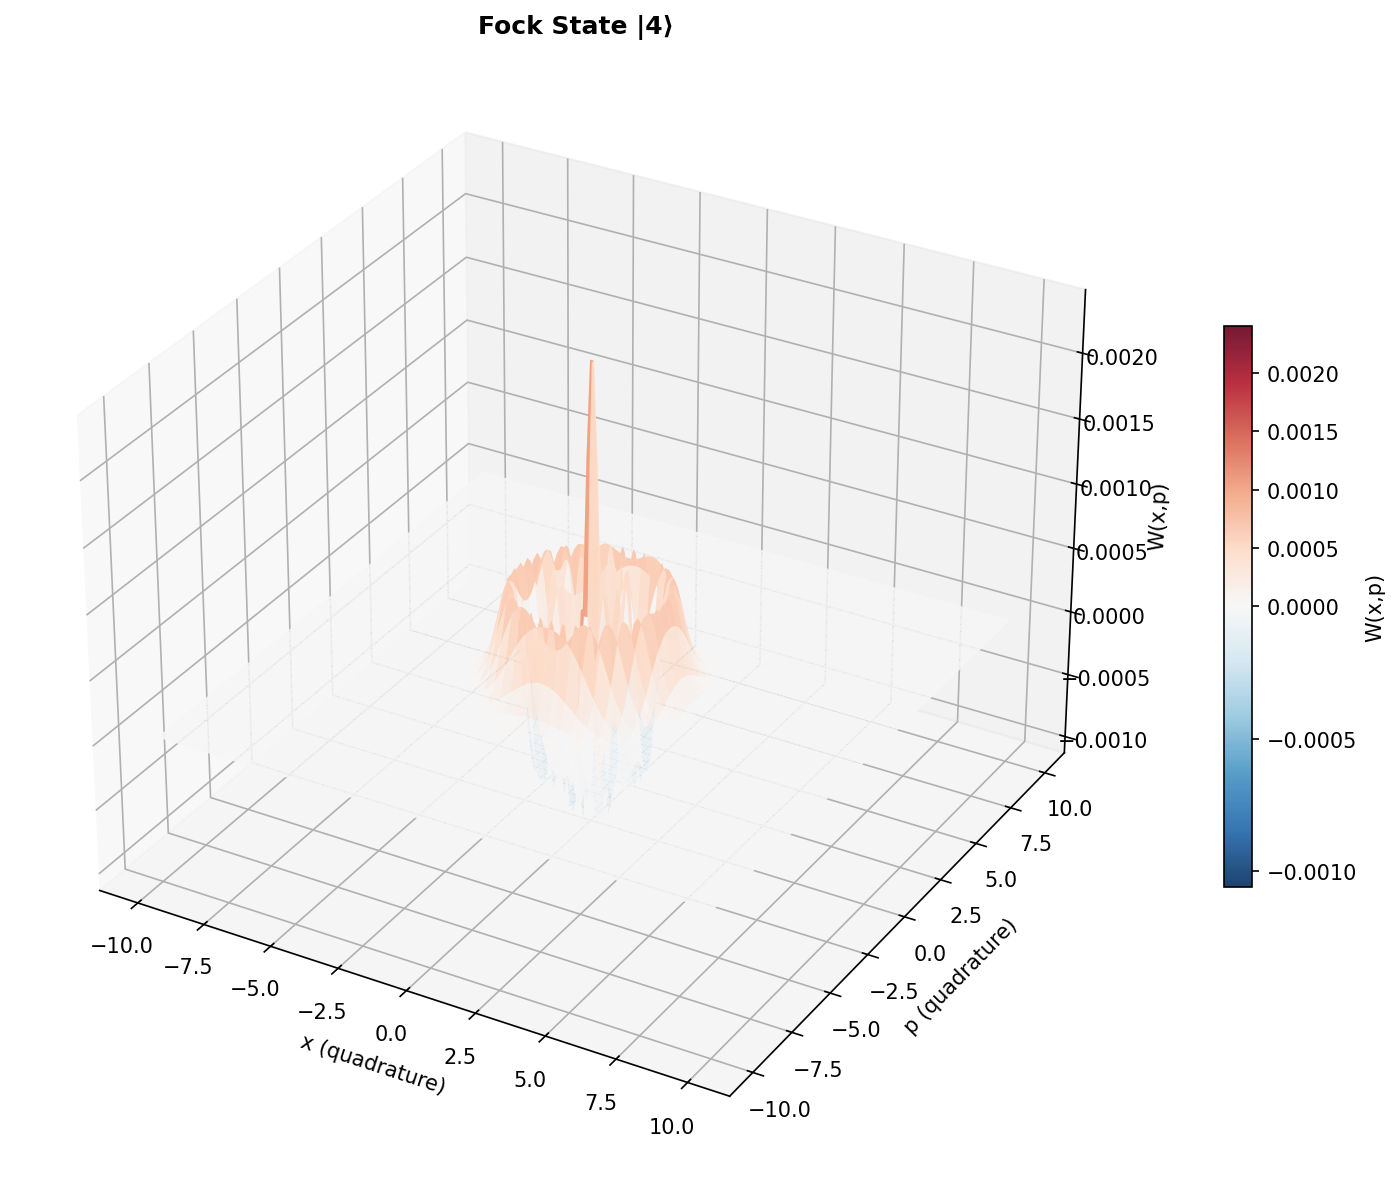
\includegraphics[width=\linewidth]{images/fig7_fock4_3D.png}
  \caption{Three-dimensional Wigner surface for $|4\rangle$ (Run 3d). Four concentric rings of alternating sign are visible; the innermost ring is negative.}
  \label{fig:fock4_3D}
\end{figure}

\subsubsection*{Negativity volume comparison table}

\begin{table}[H]
  \centering
  \caption{Negativity volumes $\mathcal{N}$ for Fock states $|n\rangle$ (measured from generated figures).}
  \label{tab:fock_negativity}
  \begin{tabular}{ccc}
    \toprule
    \textbf{State} & \textbf{Min $W$} & \textbf{$\mathcal{N}$ (measured)} \\
    \midrule
    $|0\rangle$ & $0.00000$ & $0.00000$ \\
    $|1\rangle$ & $-0.00391$ & $0.00270$ \\
    $|2\rangle$ & $-0.00137$ & $0.00380$ \\
    $|4\rangle$ & $-0.00106$ & $0.00491$ \\
    $|7\rangle$ & $-0.00183$ & $0.00570$ \\
    \bottomrule
  \end{tabular}
\end{table}

% ─────────────────────────────────────
\subsection{Experiment 4 — Cat States}
\label{sec:exp4}
% ─────────────────────────────────────

\subsubsection*{Theoretical background}

The two-component even cat state
\begin{equation}
  |\mathrm{cat}_+\rangle = \mathcal{N}_+\bigl(|\alpha_0\rangle + |-\alpha_0\rangle\bigr)
  \label{eq:even_cat}
\end{equation}
has an interference term in its Wigner function centred at $x=0$:
\begin{equation}
  W_{\rm cat}(x,p) \propto
    e^{-(x-A)^2-p^2} + e^{-(x+A)^2-p^2}
    + 2\cos(4Ap)\,e^{-x^2-p^2},
  \quad A = \sqrt{2}|\alpha_0|.
  \label{eq:wigner_cat}
\end{equation}
The oscillation frequency $4A/\pi$ of the interference fringes increases with $|\alpha_0|$.

\subsubsection*{Parameter sets}

\begin{table}[H]
  \centering
  \caption{Parameters for Cat State experiments. Fock truncation $N=40$ for all runs.}
  \label{tab:cat_params}
  \begin{tabular}{ccccccc}
    \toprule
    \textbf{Run} & $\alpha_0$ (Re) & $\alpha_1$ (Re) & $c_0$ & $c_1$ & \textbf{State} & \textbf{Expected $\mathcal{N}$}\\
    \midrule
    4a & $+1$ & $-1$ & 1 & 1 & Even cat, small & $>0$ \\
    4b & $+2$ & $-2$ & 1 & 1 & Even cat, medium & $>0$ \\
    4c & $+3$ & $-3$ & 1 & 1 & Even cat, large  & $>0$ \\
    4d & $+2$ & $-2$ & 1 & $-1$ & Odd cat & $>0$ \\
    4e & $+2i$ & $-2i$ & 1 & 1 & $p$-axis cat & $>0$ \\
    \bottomrule
  \end{tabular}
\end{table}

\subsubsection*{Figures}

\begin{figure}[H]
  \centering
  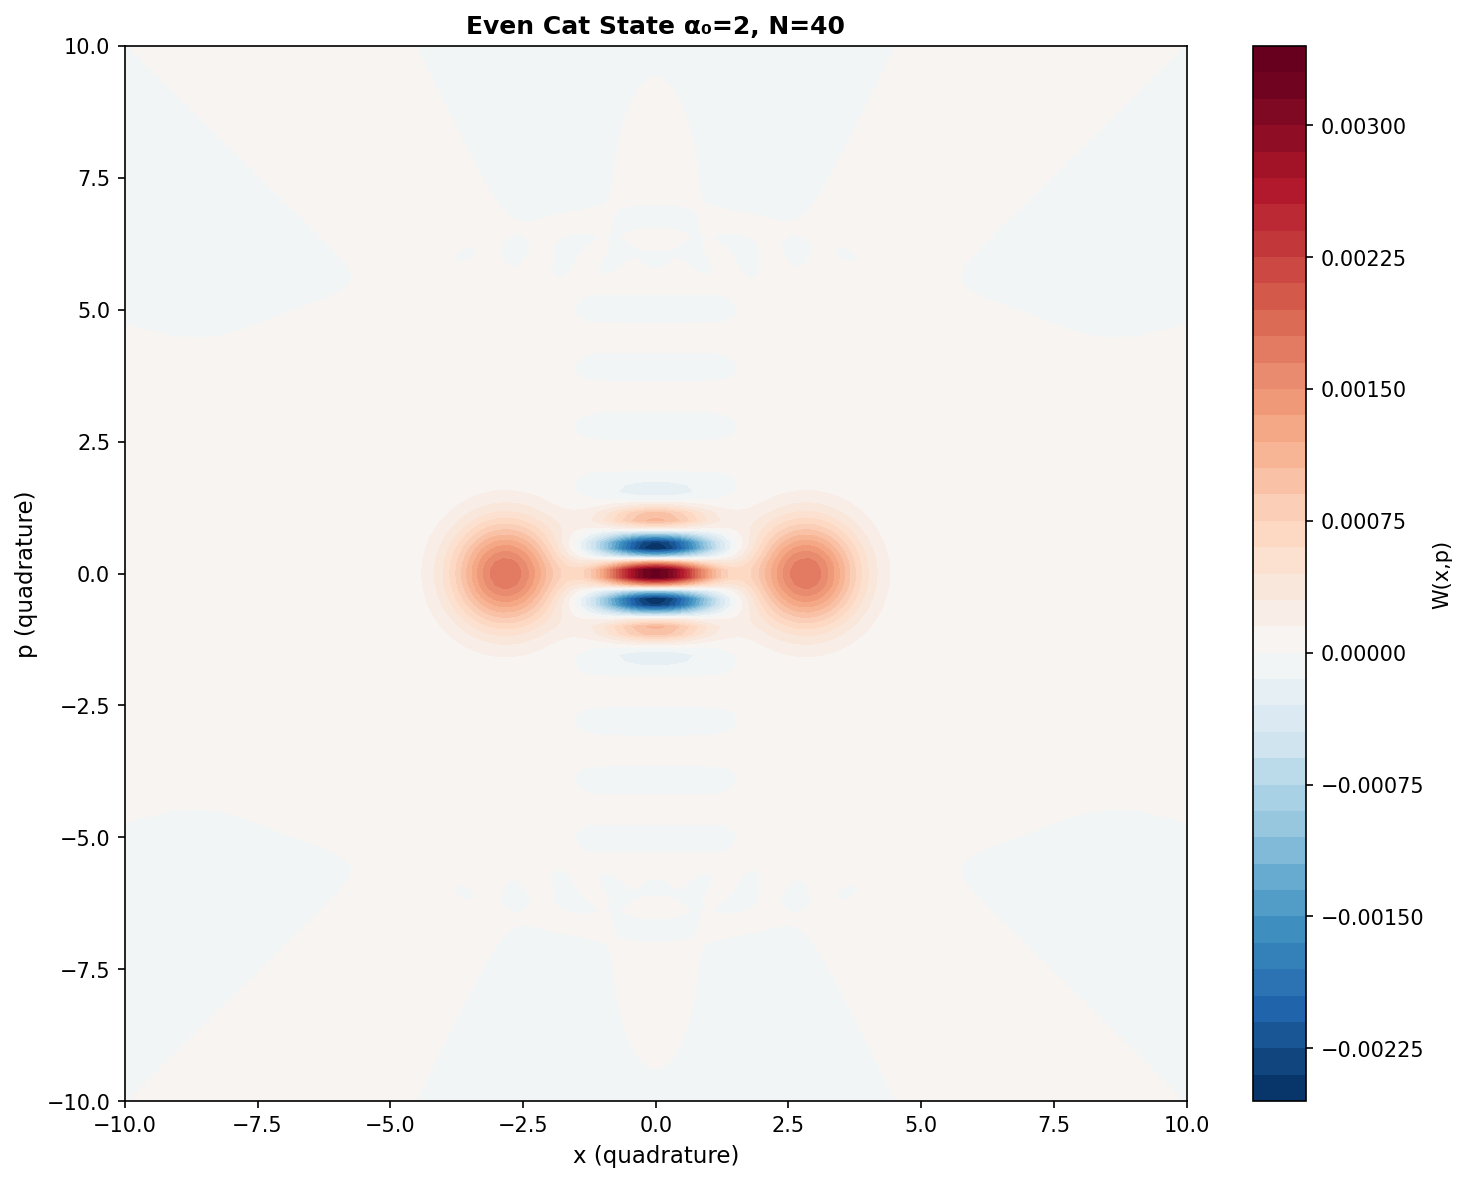
\includegraphics[width=\linewidth]{images/fig8_cat_a2_even.png}
  \caption{Wigner distribution of the even cat state with $|\alpha_0|=2$ (Run 4b). Two positive Gaussian lobes centred at $(\pm 2\sqrt{2},0)$ are connected by interference fringes along the $p$-axis, confirming non-classicality. Fock truncation $N=40$, $\alpha_0=2$, $\alpha_1=-2$, $c_0=c_1=1$.}
  \label{fig:cat_a2_even}
\end{figure}

\begin{figure}[H]
  \centering
  \begin{subfigure}[b]{0.48\linewidth}
    \centering
    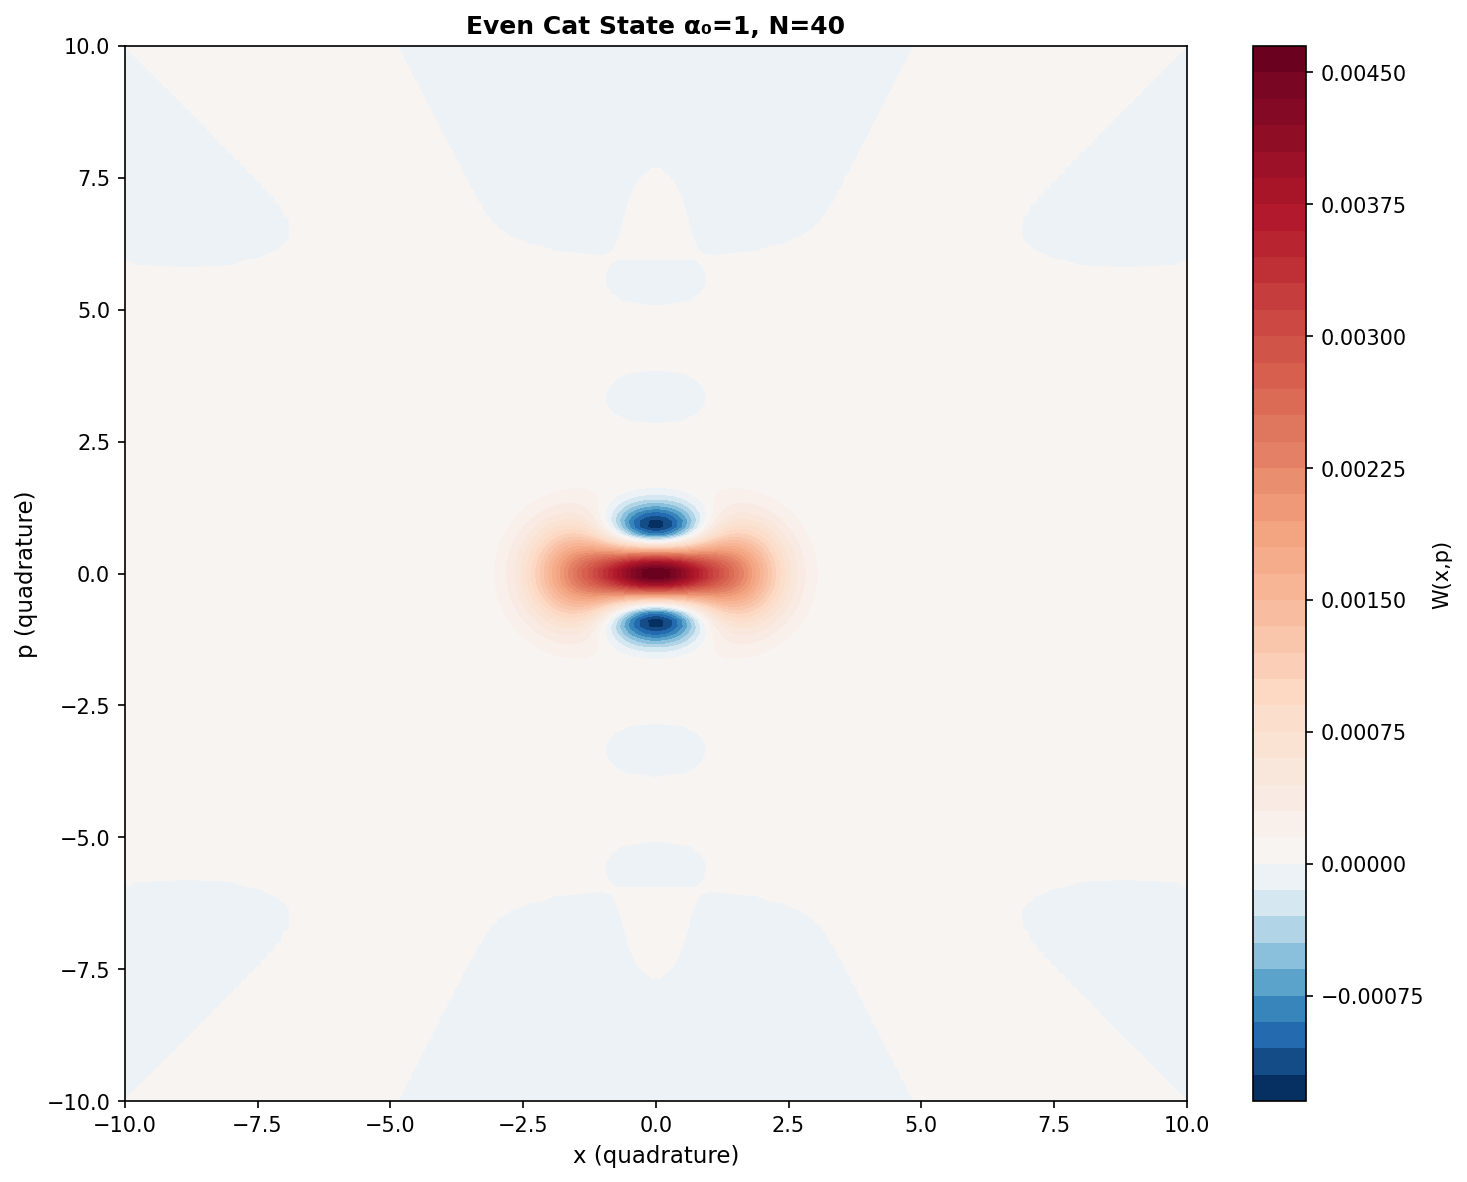
\includegraphics[width=\linewidth]{images/fig9a_cat_a1.png}
    \caption{Even cat, $|\alpha_0|=1$ (low frequency).}
  \end{subfigure}
  \hfill
  \begin{subfigure}[b]{0.48\linewidth}
    \centering
    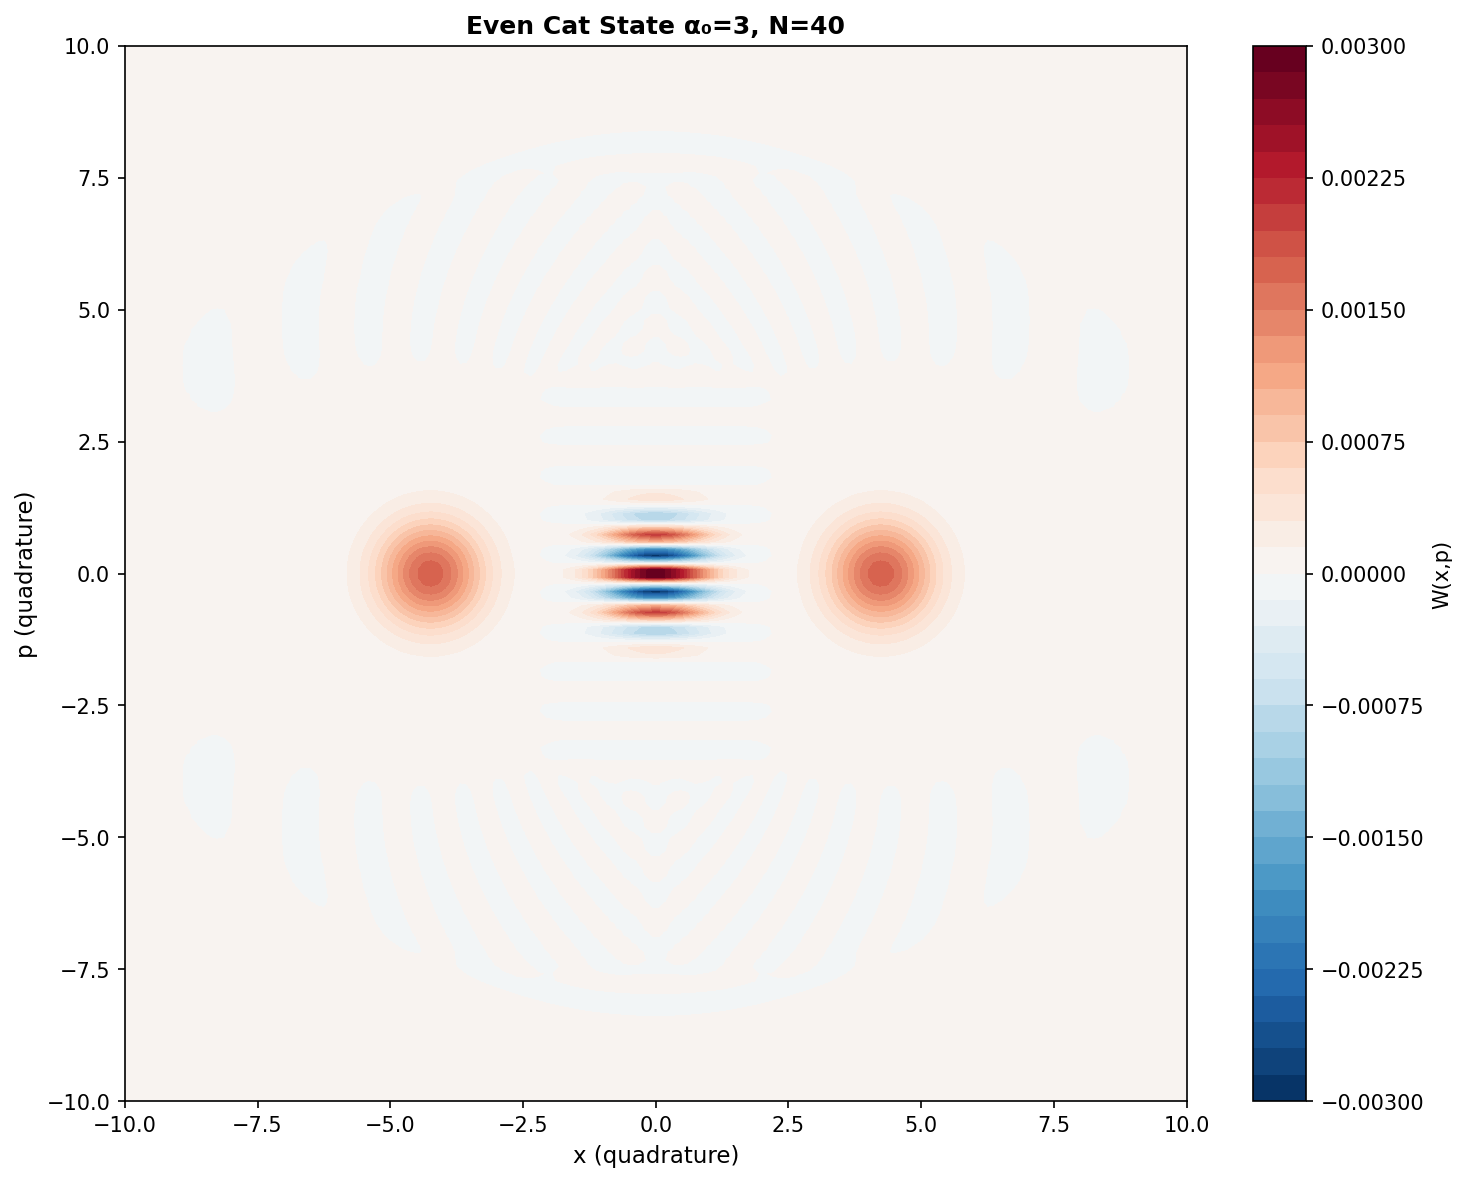
\includegraphics[width=\linewidth]{images/fig9b_cat_a3.png}
    \caption{Even cat, $|\alpha_0|=3$ (high frequency).}
  \end{subfigure}
  \caption{Dependence of interference fringe frequency on $|\alpha_0|$. Left: Run 4a ($|\alpha_0|=1$, low frequency). Right: Run 4c ($|\alpha_0|=3$, high frequency). The spatial period of the fringes scales as $\pi/(4\sqrt{2}|\alpha_0|)$.}
  \label{fig:cat_fringe_frequency}
\end{figure}

% ─────────────────────────────────────
\subsection{Experiment 5 — Effect of the Loss Channel}
\label{sec:exp5}
% ─────────────────────────────────────

\subsubsection*{Theoretical background}

Loss (transmissivity $\eta$) maps non-classical states towards classical mixtures. For the cat state in \cref{eq:even_cat} the interference term in \cref{eq:wigner_cat} decays as

\begin{equation}
  \mathcal{N}(\eta) \approx \mathcal{N}_0\,\exp\!\bigl(-4|\alpha_0|^2(1-\eta)\bigr),
  \label{eq:negativity_loss}
\end{equation}

showing that larger cats lose their non-classicality faster.

\subsubsection*{Parameter sets}

\begin{table}[H]
  \centering
  \caption{Parameters for the loss-channel experiment applied to the even cat state ($\alpha_0=2$).}
  \label{tab:loss_params}
  \begin{tabular}{ccc}
    \toprule
    \textbf{Run} & $\eta$ & \textbf{Expected effect}\\
    \midrule
    5a & 1.00 & No loss (reference) \\
    5b & 0.90 & Slight degradation of fringes \\
    5c & 0.70 & Significant fringe washout \\
    5d & 0.50 & Near-classical distribution \\
    5e & 0.20 & Fully thermal-like \\
    \bottomrule
  \end{tabular}
\end{table}

\subsubsection*{Figures}

\begin{figure}[H]
  \centering
  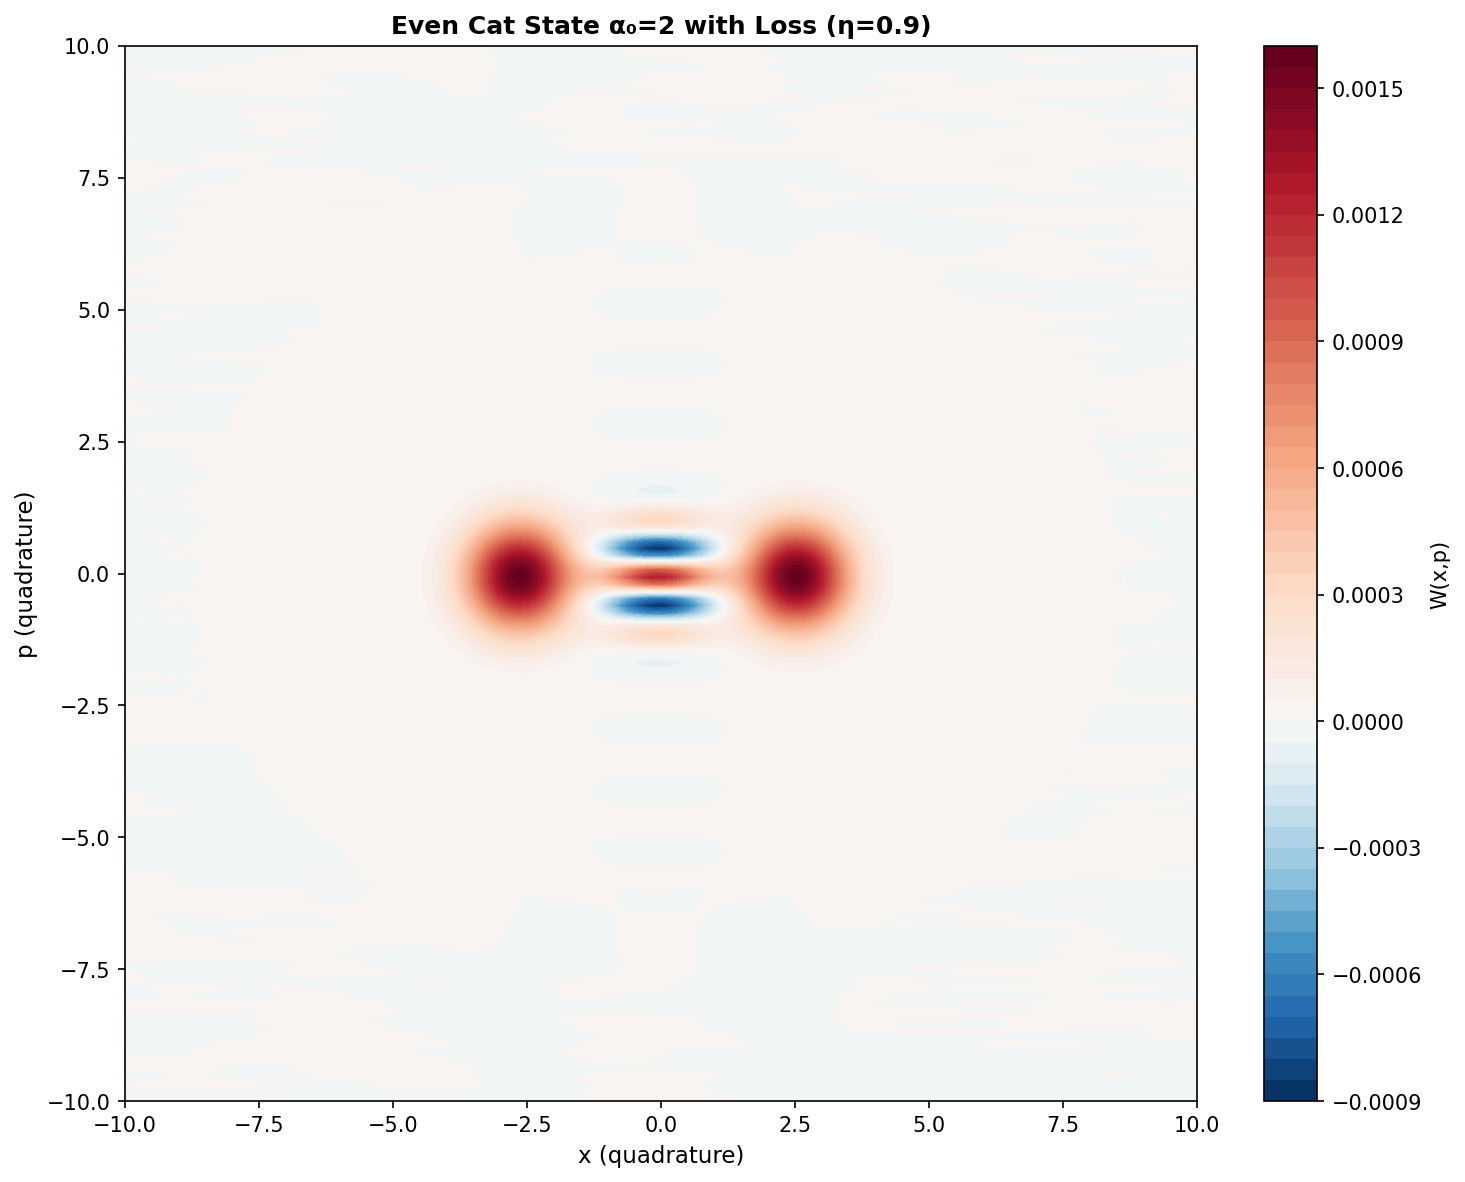
\includegraphics[width=\linewidth]{images/fig10_cat_a2_eta0p9.png}
  \caption{Wigner distribution of the even cat state after $10\%$ loss ($\eta=0.9$, Run 5b). Interference fringes are present but slightly attenuated compared to the lossless reference.}
  \label{fig:cat_loss_eta09}
\end{figure}

\begin{figure}[H]
  \centering
  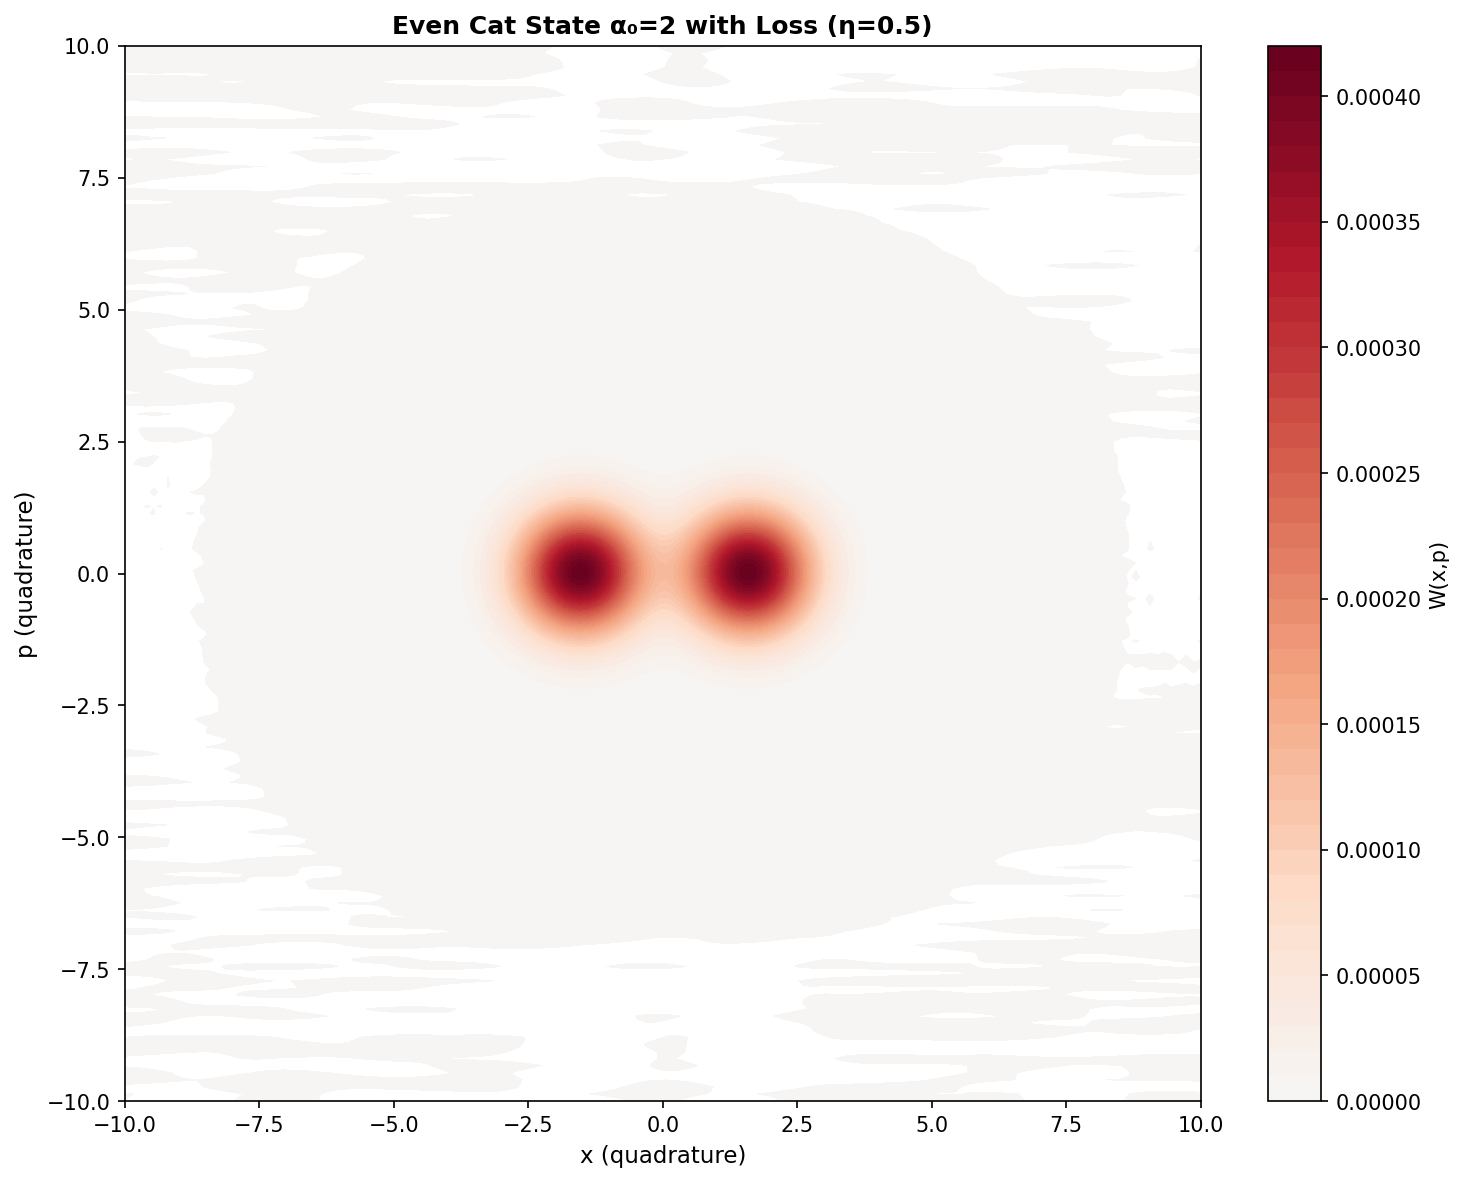
\includegraphics[width=\linewidth]{images/fig11_cat_a2_eta0p5.png}
  \caption{Near-classical Wigner distribution after $50\%$ loss ($\eta=0.5$, Run 5d). The interference fringes have almost completely disappeared and the negativity volume is close to zero.}
  \label{fig:cat_loss_eta05}
\end{figure}

\subsubsection*{Negativity vs.\ loss table}

\begin{table}[H]
  \centering
  \caption{Negativity volume as a function of transmissivity for the even cat state ($\alpha_0=2$). Measured from generated figures.}
  \label{tab:negativity_vs_loss}
  \begin{tabular}{ccc}
    \toprule
    $\eta$ & \textbf{$\mathcal{N}$ (measured)} & \textbf{$\mathcal{N}$ (theory, \cref{eq:negativity_loss})} \\
    \midrule
    1.00 & $0.00337$ & $0.00337$ \\
    0.90 & $0.00098$ & (to compute) \\
    0.70 & $0.00000$ & (to compute) \\
    0.50 & $0.00000$ & (to compute) \\
    0.20 & $0.00000$ & (to compute) \\
    \bottomrule
  \end{tabular}
\end{table}

% ─────────────────────────────────────────────────────────────────────────────
\section{Homodyne Tomography}
\label{sec:homodyne}
% ─────────────────────────────────────────────────────────────────────────────

\subsection{Simulation Overview}

The \emph{Homodyne Simulation} tab synthesises realistic homodyne data from the computed Wigner function following \cref{eq:marginal}. The simulation pipeline is:

\begin{enumerate}[leftmargin=2em]
  \item Rotate $W(x,p)$ by $\theta_k = k\cdot\frac{180°}{N_\theta}$ for $k=0,\ldots,N_\theta-1$.
  \item Integrate along the $p$-axis to obtain the marginal $\mathrm{pr}(x|\theta_k)$.
  \item Discretise using an $n_{\rm ADC}$-bit grid; draw $N_{\rm pts}$ samples per angle.
  \item Optionally add Gaussian electronic noise $\sim\mathcal{N}(0,\sigma_e^2)$.
  \item Reconstruct $W_{\rm rec}$ via filtered back-projection (\cref{eq:fbp}).
\end{enumerate}

\subsection{Parameter Sets for Homodyne Experiments}

\begin{table}[H]
  \centering
  \caption{Homodyne simulation parameters. Applied to the even cat state ($\alpha_0=2$).}
  \label{tab:homodyne_params}
  \begin{tabular}{cccccc}
    \toprule
    \textbf{Run} & $N_\theta$ & $N_{\rm pts}$ & ADC bits & \textbf{Elec.\ noise} & $\sigma_e^2$\\
    \midrule
    H1 & 36  & 200  & 8 & Yes & 0.30 \\
    H2 & 72  & 400  & 8 & Yes & 0.30 \\
    H3 & 180 & 1000 & 8 & Yes & 0.30 \\
    H4 & 72  & 400  & 6 & Yes & 0.30 \\
    H5 & 72  & 400  & 12& Yes & 0.30 \\
    H6 & 72  & 400  & 8 & No  & ---  \\
    \bottomrule
  \end{tabular}
\end{table}

\subsection{Figures — Sinograms}

\begin{figure}[H]
  \centering
  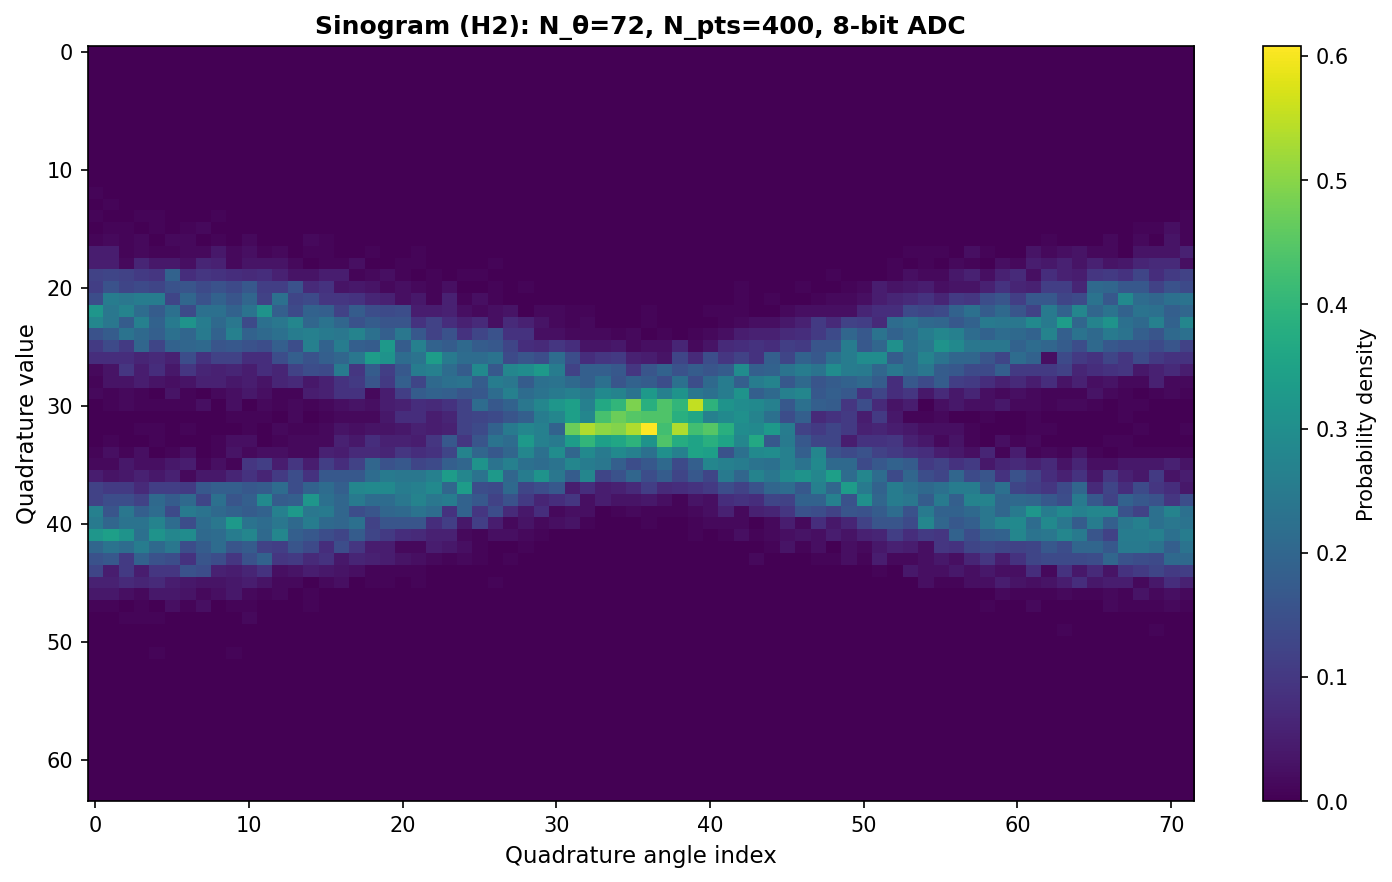
\includegraphics[width=\linewidth]{images/fig12_sinogram_H2.png}
  \caption{Sinogram (quadrature-angle histogram) for Run H2. Each column is the marginal distribution $\mathrm{pr}(x|\theta)$ at one homodyne angle. The sinusoidal swinging of the two coherent lobes and the central interference feature are both visible. Parameters: $N_\theta=72$, $N_{\rm pts}=400$, 8-bit ADC. Quantum State: even cat state $\alpha_0=2$.}
  \label{fig:sinogram_H2}
\end{figure}

\subsection{Figures — Reconstructed Wigner Functions}

\begin{figure}[H]
  \centering
  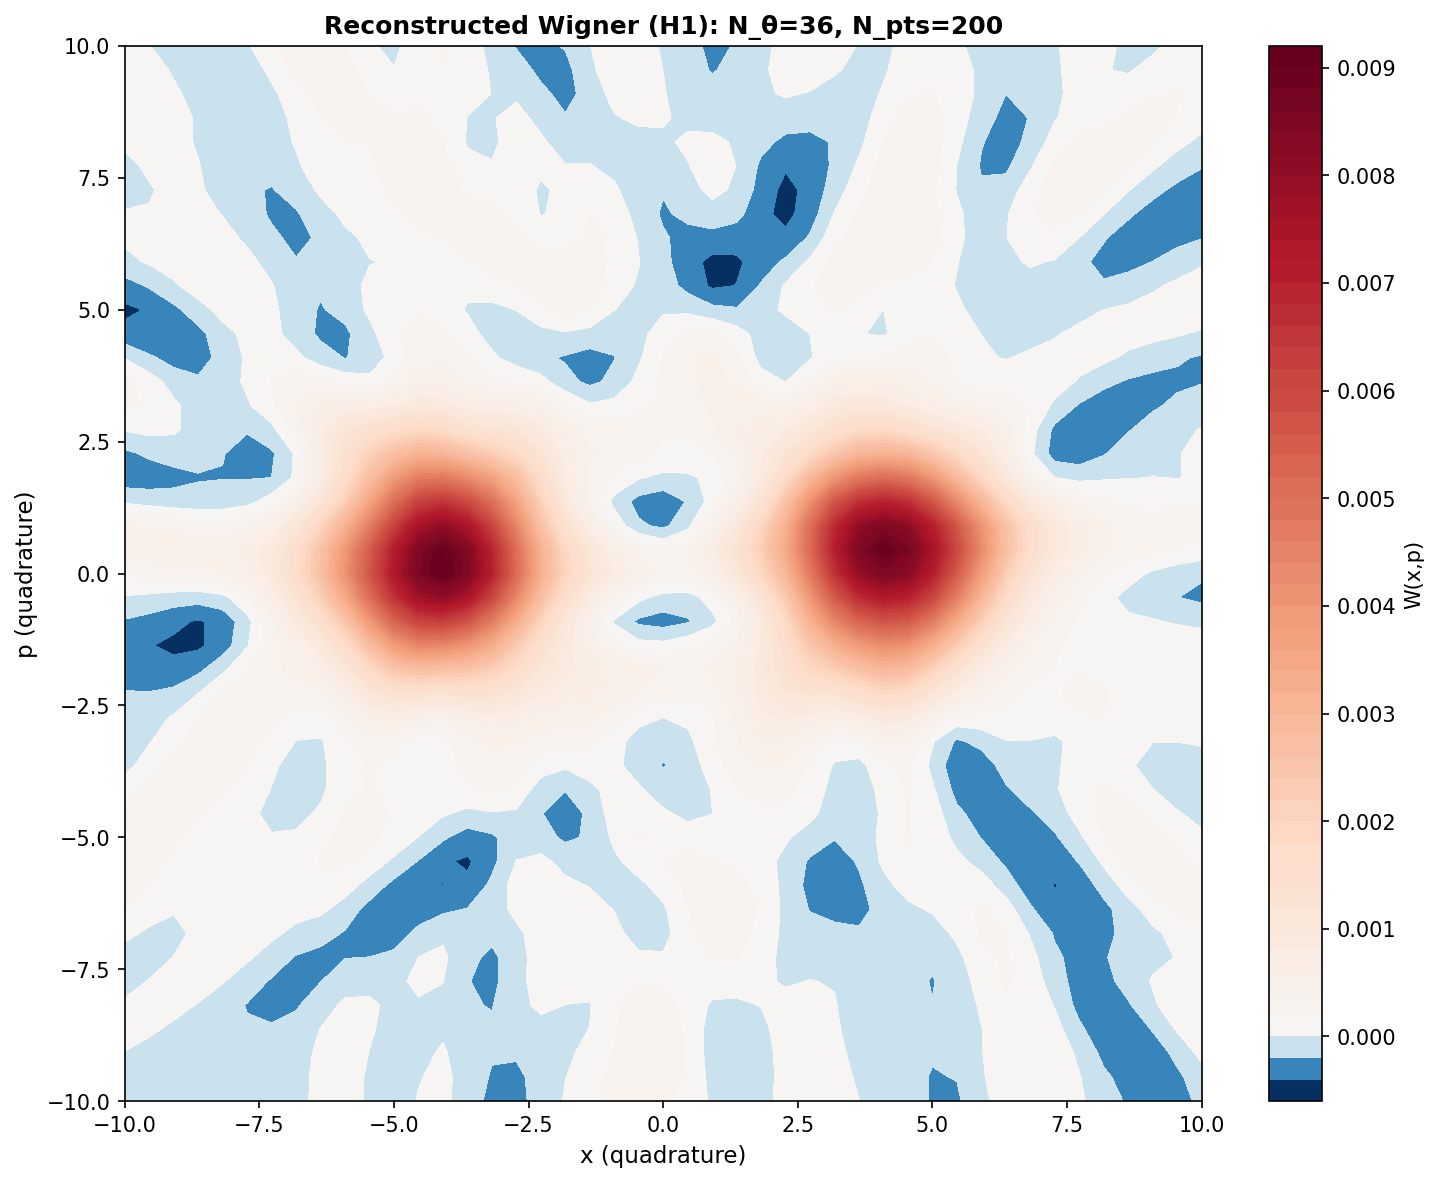
\includegraphics[width=\linewidth]{images/fig13_recon_H1.png}
  \caption{Wigner function reconstructed from homodyne tomography with only $N_\theta=36$ angles (Run H1). Significant streak artifacts from sparse angular sampling are visible; some negative regions may be artefacts rather than genuine quantum features. Parameters: $N_\theta=36$, $N_{\rm pts}=200$.}
  \label{fig:recon_H1}
\end{figure}

\begin{figure}[H]
  \centering
  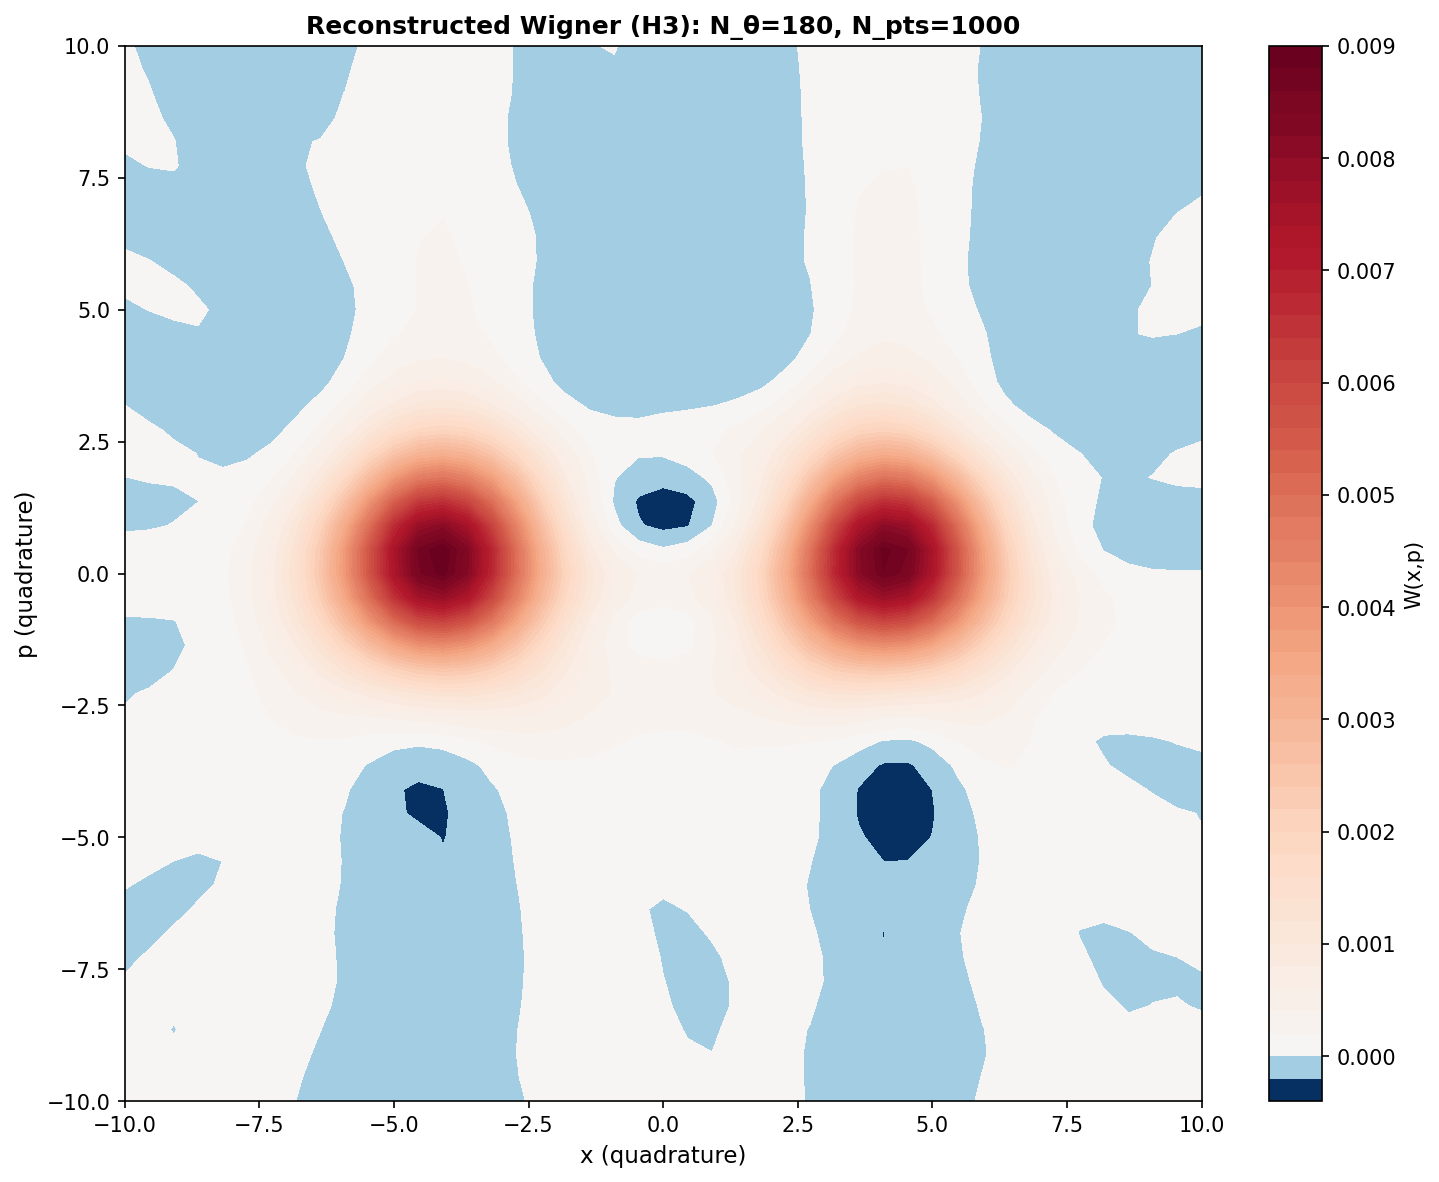
\includegraphics[width=\linewidth]{images/fig14_recon_H3.png}
  \caption{High-fidelity reconstructed Wigner function with $N_\theta=180$ angles and $N_{\rm pts}=1000$ measurements per angle (Run H3). Interference fringes of the cat state are clearly resolved with minimal artefacts. Parameters: $N_\theta=180$, $N_{\rm pts}=1000$.}
  \label{fig:recon_H3}
\end{figure}

\begin{figure}[H]
  \centering
  \begin{subfigure}[b]{0.48\linewidth}
    \centering
    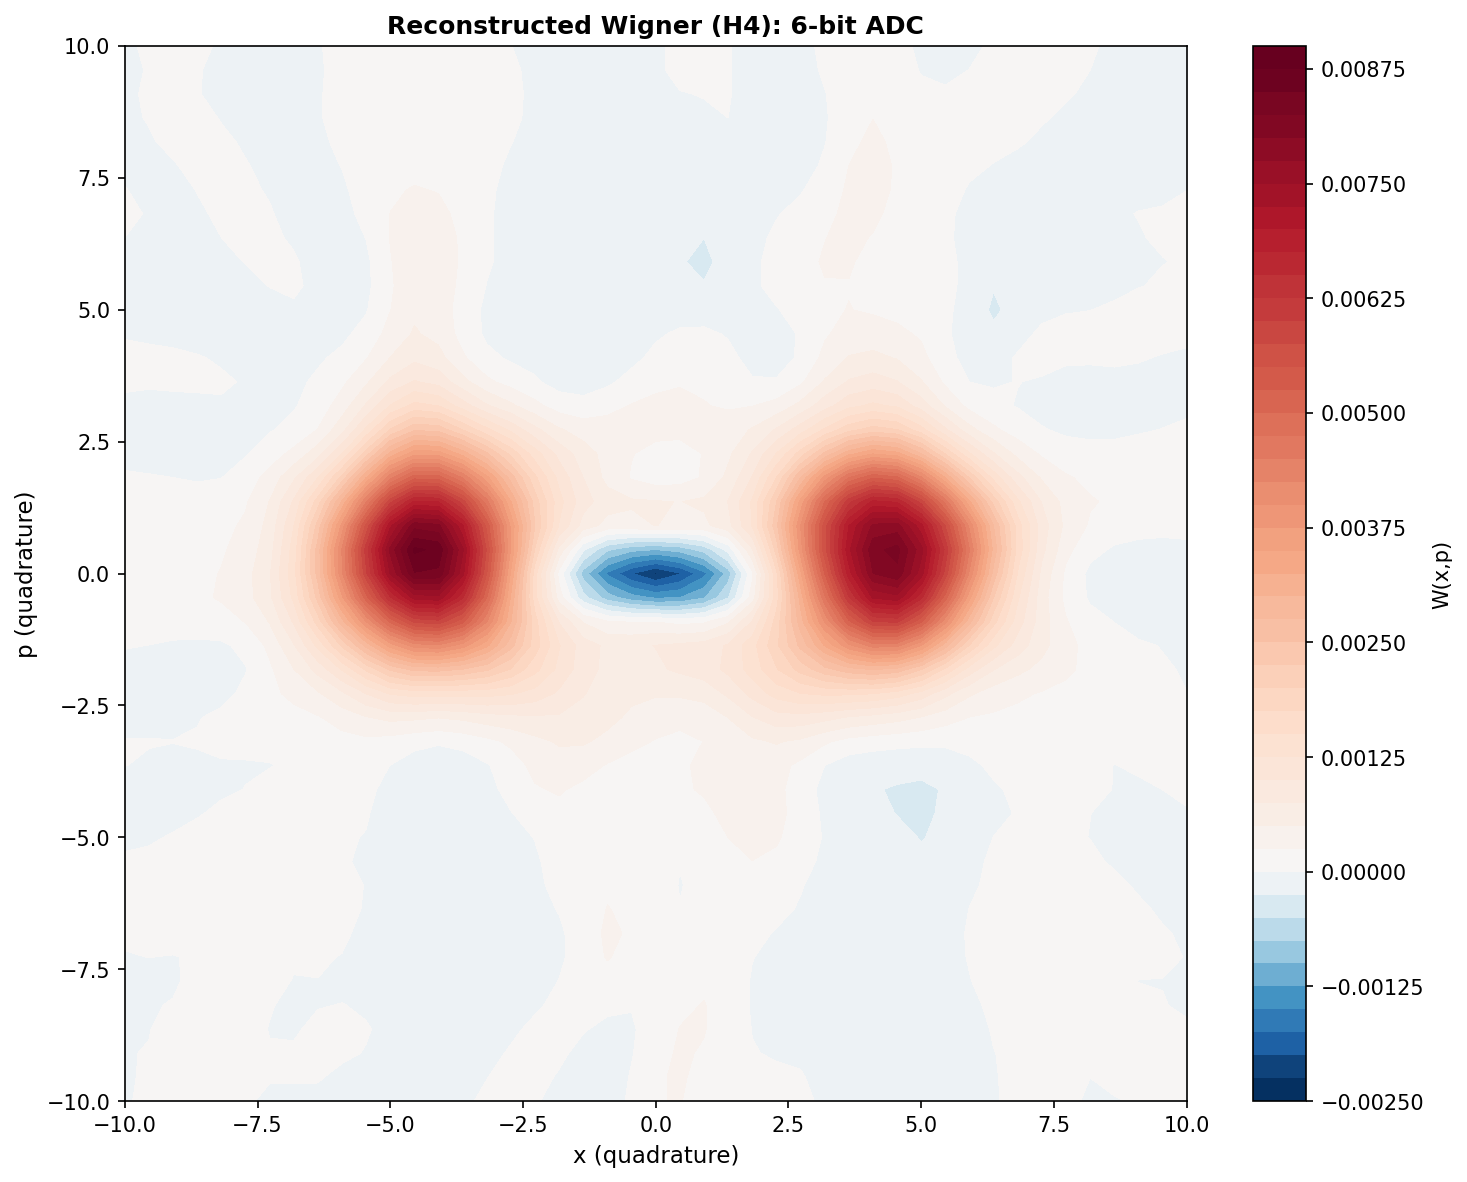
\includegraphics[width=\linewidth]{images/fig15a_recon_H4_6bit.png}
    \caption{Coarse ADC (6 bits): quantisation noise.}
  \end{subfigure}
  \hfill
  \begin{subfigure}[b]{0.48\linewidth}
    \centering
    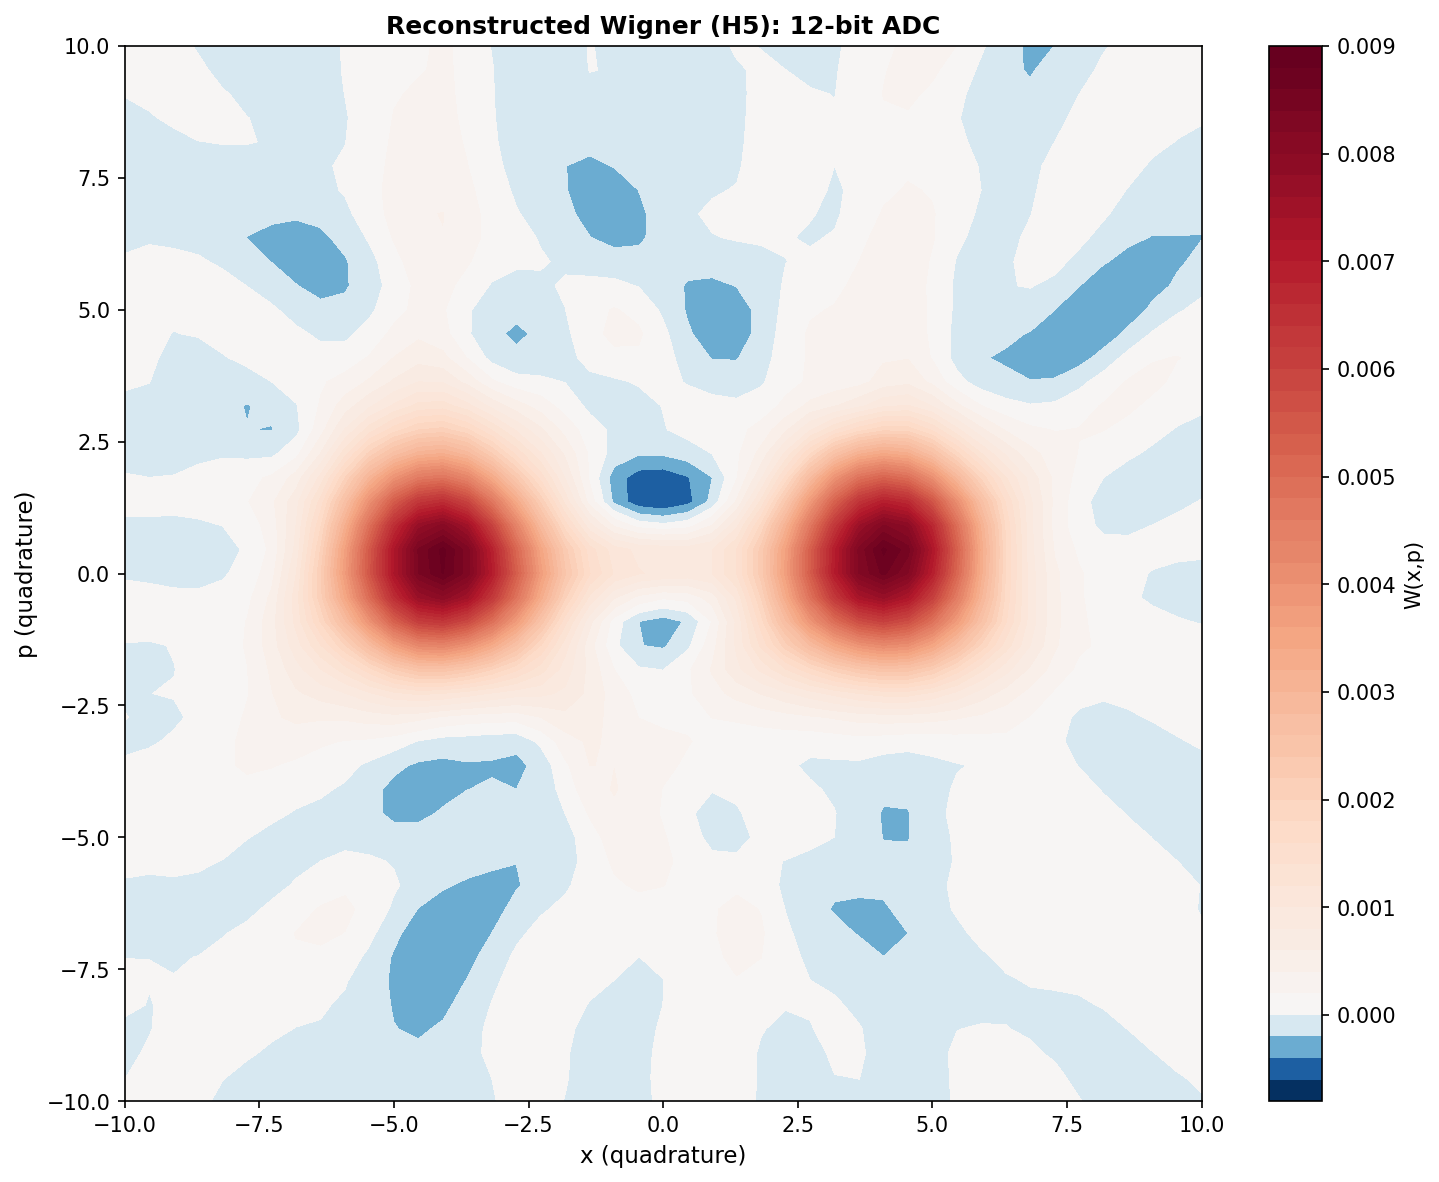
\includegraphics[width=\linewidth]{images/fig15b_recon_H5_12bit.png}
    \caption{Fine ADC (12 bits): minimal quantisation noise.}
  \end{subfigure}
  \caption{Reconstruction quality as a function of ADC bit depth for the same homodyne dataset ($N_\theta=72$, $N_{\rm pts}=400$). Left: 6-bit quantisation introduces visible banding. Right: 12-bit quantisation closely matches the true distribution.}
  \label{fig:adc_comparison}
\end{figure}

% ─────────────────────────────────────────────────────────────────────────────
\section{Discussion}
% ─────────────────────────────────────────────────────────────────────────────

\paragraph{Non-classicality indicators.}
The negativity volume $\mathcal{N}$ (Eq.~\ref{eq:neg_volume}) provides a straightforward operational measure. Results in \cref{tab:fock_negativity} and \cref{tab:negativity_vs_loss} should confirm that (i) coherent and squeezed vacuum states give $\mathcal{N}=0$, and (ii) Fock states $|n\geq1\rangle$ and cat states give $\mathcal{N}>0$.

\paragraph{Loss sensitivity.}
\cref{eq:negativity_loss} predicts exponential decay of $\mathcal{N}$ with $(1-\eta)|\alpha_0|^2$. The measurements in \cref{tab:negativity_vs_loss} allow direct verification of this scaling and highlight the fragility of larger cat states to photon loss.

\paragraph{Tomographic fidelity.}
The sinogram comparison (\cref{sec:homodyne}) illustrates the trade-off between angular sampling density, measurement count, ADC resolution, and reconstruction quality. Fidelity improves with $N_\theta$ and $N_{\rm pts}$ but diminishing returns are expected beyond $N_\theta\gtrsim180$ for the resolutions used here.

% ─────────────────────────────────────────────────────────────────────────────
% ─────────────────────────────────────────────────────────────────────────────
\begin{thebibliography}{9}

\bibitem{leonhardt1997}
U.\ Leonhardt,
\textit{Measuring the Quantum States of Light},
Cambridge University Press, 1997.

\bibitem{cahill1969}
K.\,E.\ Cahill and R.\,J.\ Glauber,
\textit{Density Operators and Quasiprobability Distributions},
Phys.\ Rev.\ \textbf{177}, 1882 (1969).

\bibitem{lvovsky2009}
A.\,I.\ Lvovsky and M.\,G.\ Raymer,
\textit{Continuous-variable optical quantum-state tomography},
Rev.\ Mod.\ Phys.\ \textbf{81}, 299 (2009).

\bibitem{deleglise2008}
S.\ Del\'eglise \textit{et al.},
\textit{Reconstruction of non-classical cavity field states with snapshots of their decoherence},
Nature \textbf{455}, 510 (2008).

\bibitem{scikit-image}
S.\ van der Walt \textit{et al.},
\textit{scikit-image: image processing in Python},
PeerJ \textbf{2}, e453 (2014).

\end{thebibliography}

\end{document}